\documentclass[11pt]{article}

% arXiv-style preprint layout
\usepackage[T1]{fontenc}
\usepackage{amsmath}
\usepackage{newtxtext,newtxmath}
\usepackage[letterpaper, margin=1in, headheight=14pt]{geometry}
\usepackage{microtype}
\usepackage{booktabs}
\usepackage[table]{xcolor}
\usepackage{caption}
\usepackage{placeins}
\usepackage{enumitem}
\usepackage{titlesec}
\usepackage{fancyhdr}
\usepackage{pgfplots}
\pgfplotsset{compat=1.18}
\usepgfplotslibrary{groupplots}
\usepackage{tikz}
\usetikzlibrary{positioning,arrows.meta,fit,decorations.pathreplacing,calc}
\usepackage[colorlinks=true,linkcolor=blue!55!black,citecolor=blue!55!black,urlcolor=blue!55!black]{hyperref}

% Colors and TikZ styles shared by the report figures.
\colorlet{cin}{black!60}
\colorlet{ccell}{blue!70!black}
\colorlet{ccol}{green!50!black}
\colorlet{cref}{orange!85!black}
\colorlet{crow}{red!65!black}
\colorlet{cicl}{yellow!55!orange}
\colorlet{cdec}{violet!75!black}
\colorlet{cdata}{teal!70!black}
\colorlet{cgpu}{green!45!black}
\tikzset{
  panel/.style={draw=#1!45, fill=#1!5, rounded corners=4pt, line width=0.6pt},
  ptitle/.style={font=\bfseries\scriptsize, anchor=north west, text=#1!85!black, inner sep=0pt},
  psub/.style={font=\tiny, anchor=north west, text=black!60, align=left, inner sep=0pt},
  sbox/.style={draw=#1!60, fill=#1!13, rounded corners=2pt, font=\tiny, align=center,
               inner sep=2pt, line width=0.4pt},
  tok/.style={draw=black!45, fill=#1, minimum size=0.21cm, inner sep=0pt, line width=0.3pt},
  flow/.style={-{Stealth[length=1.5mm]}, line width=0.5pt, black!70},
  bigflow/.style={-{Stealth[length=2.6mm,width=2.2mm]}, line width=1.1pt, black!70},
  shapelabel/.style={font=\tiny, text=black!80, align=center},
  note/.style={font=\tiny, text=black!65, align=center},
  plus/.style={circle, draw=black!60, fill=white, inner sep=0pt, minimum size=0.26cm, font=\tiny},
  eq/.style={font=\scriptsize, align=center, text width=3.65cm},
  dim/.style={font=\tiny, text=black!75, inner sep=1pt},
  stitle/.style={font=\bfseries\footnotesize, anchor=north west, text=#1!85!black, inner sep=0pt},
}
% \tensor{x}{y}{w}{h}{d}{color}: an n x m x d block, front face w x h, depth d drawn obliquely
\newcommand{\tensor}[6]{%
  \filldraw[fill=#6!14, draw=#6!75!black, line width=0.45pt] (#1,#2) rectangle ({#1+#3},{#2+#4});
  \filldraw[fill=#6!28, draw=#6!75!black, line width=0.45pt] (#1,{#2+#4}) -- ({#1+0.6*#5},{#2+#4+0.45*#5})
    -- ({#1+#3+0.6*#5},{#2+#4+0.45*#5}) -- ({#1+#3},{#2+#4}) -- cycle;
  \filldraw[fill=#6!40, draw=#6!75!black, line width=0.45pt] ({#1+#3},#2) -- ({#1+#3+0.6*#5},{#2+0.45*#5})
    -- ({#1+#3+0.6*#5},{#2+#4+0.45*#5}) -- ({#1+#3},{#2+#4}) -- cycle;}
% \matrixbox{x}{y}{w}{h}{color}: a plain matrix
\newcommand{\matrixbox}[5]{%
  \filldraw[fill=#5!14, draw=#5!75!black, line width=0.45pt] (#1,#2) rectangle ({#1+#3},{#2+#4});}


\captionsetup{font=small,labelfont=bf,labelsep=period}
\setlength{\tabcolsep}{5pt}
\renewcommand{\topfraction}{0.92}
\renewcommand{\bottomfraction}{0.6}
\renewcommand{\textfraction}{0.06}
\renewcommand{\floatpagefraction}{0.75}
\setcounter{topnumber}{3}
\setcounter{totalnumber}{5}
\setlist{itemsep=2pt, topsep=4pt}
\titleformat{\section}{\large\bfseries}{\thesection}{0.8em}{}
\titleformat{\subsection}{\normalsize\bfseries}{\thesubsection}{0.8em}{}
\titlespacing*{\section}{0pt}{14pt plus 3pt minus 2pt}{6pt plus 2pt}
\titlespacing*{\subsection}{0pt}{10pt plus 2pt minus 2pt}{4pt plus 1pt}
\titlespacing*{\paragraph}{0pt}{6pt plus 2pt}{0.8em}

\pagestyle{fancy}
\fancyhf{}
\fancyhead[L]{\small\scshape A sling against giants}
\fancyhead[R]{\small\scshape Technical report, version 1.0, October 2026}
\fancyfoot[C]{\small\thepage}
\renewcommand{\headrulewidth}{0.4pt}
\fancypagestyle{plain}{\fancyhf{}\fancyfoot[C]{\small\thepage}\renewcommand{\headrulewidth}{0pt}}

\newcommand{\R}{\mathbb{R}}
\newcommand{\E}{\mathbb{E}}
\newcommand{\Dc}{\mathcal{D}_{\mathrm{ctx}}}
\newcommand{\Block}{\operatorname{Block}}
\newcommand{\Attn}{\operatorname{Attn}}
\newcommand{\LN}{\operatorname{LN}}
\newcommand{\RMS}{\operatorname{RMSNorm}}

\hypersetup{pdftitle={A Sling Against Giants: LightPFN, a 4.6M-parameter tabular in-context classifier designed to stay small},
            pdfauthor={Giorgio Ottoboni}}

\begin{document}

\thispagestyle{plain}
\begin{center}
\rule{\linewidth}{1.6pt}\\[10pt]
{\LARGE\bfseries A Sling Against Giants\par}
\vspace{6pt}
{\Large LightPFN, a 4.6M-parameter tabular in-context classifier\\designed to stay small\par}
\vspace{8pt}
\rule{\linewidth}{0.6pt}\\[14pt]
{\large Giorgio Ottoboni}\\[4pt]
{\small Technical report, version 1.0, 8 October 2026}\\[2pt]
{\small\url{https://github.com/GioOtto/LightPFN}}
\end{center}
\vspace{6pt}

\begin{abstract}
We present LightPFN, a tabular in-context classifier with 4.60 million parameters, pretrained exclusively
on synthetic tasks without distillation. Its three-stage architecture combines summary-mediated row
refinement with a target-aware column stage; pretraining mixes structural causal graph and rule priors.
Model selection uses held-out synthetic tasks, mechanism probes and real datasets outside TabArena.
The final model achieves a mean AUC of 0.911 on 55 external small-table datasets, 0.9 percentage points
above default CatBoost. A long-context training stage improves performance on larger tables: mean AUC
differences from default CatBoost have 95\% bootstrap intervals including zero at 4,000--32,000 training
rows and, in a separate evaluation on larger datasets, at 10,000--100,000 rows. On 38 TabArena classification
tasks, using the official splits of one repeat, four estimators rank second among seven evaluated
configurations, behind TabICLv2, and yield lower error than default CatBoost on 76\% of tasks. A separate
run of the official TabArena-Lite pipeline on the 38 classification datasets places LightPFN 25th of 99
methods, with Elo 1420 ($+67/-66$). Its point estimate exceeds all GBDT entries, including tuned and ensembled
ones, but its interval overlaps tuned CatBoost's. This author-run Lite result awaits the maintainers' full
benchmark verification. Cache blocking and folded normalization reduce CPU inference time by
1.1--4.1 times with predictions unchanged up to floating-point rounding. Future work will assess
inference latency and memory use on less powerful computers, including laptops.
\end{abstract}

\noindent\textbf{Keywords:} tabular foundation models $\cdot$ in-context learning $\cdot$ synthetic
priors $\cdot$ small models $\cdot$ CPU inference

\section{Introduction}

Gradient-boosted decision trees remain the default choice for tabular classification. They are
widely used on CPUs and remain strong baselines after tuning. Prior-data fitted networks
(PFNs) \cite{muller2022,hollmann2023} approach the problem from a different angle: a transformer is
trained once on millions of synthetic datasets drawn from a prior over data-generating processes,
and at test time it reads a labelled training set as context and predicts the test labels in a
single forward pass. The network then approximates the posterior predictive distribution of the
prior, so the quality of the prior and the capacity of the network determine what it can learn.
TabPFN v2 \cite{hollmann2025}, TabICL \cite{qu2025} and their successors have shown that this
recipe matches or exceeds tuned boosting on public benchmarks such as TabArena \cite{tabarena},
with models ranging from a few million to several hundred million parameters, usually served on
GPU.

This report describes LightPFN, a model built under three constraints. The parameter budget stays
below five million, with the goal of keeping inference practical on a commodity CPU; a small parameter
count does not by itself ensure latency comparable to boosted trees. Training uses synthetic data only,
with no distillation and no weights or predictions of other tabular foundation models. Code, weights and the
training pipeline are released under the Apache 2.0 license (\url{https://github.com/GioOtto/LightPFN}, package
\texttt{LightPFN} on PyPI); dependency licenses still apply. Finally, after
introducing the selection protocol, design choices use sets outside TabArena, which is reserved for
evaluating the finalists. An earlier exploratory TabArena evaluation is disclosed in
Section~\ref{sec:gbdt}.

The practical target is the way boosted trees are used day to day: with default settings, on a
laptop. A model that matches or beats default CatBoost, LightGBM and XGBoost without tuning and without
a GPU is useful even where tuned and ensembled boosting stays ahead, so we report the comparison with
default tree ensembles alongside the selection sets.

Our contributions are the following.
\begin{enumerate}
  \item An adaptation and evaluation of refinement before compression \cite{causilo} under a
  sub-five-million parameter budget (Section~\ref{sec:model}). Four temporary tokens mediate
  within-row interactions, a second target-aware column stage revisits the context, and a separate
  readout compresses each row. Removing one in-context block funds the added modules: the resulting
  configuration improves held-out synthetic AUC by 0.56 points and external AUC by 0.51 points over
  the baseline, with 4.60M rather than 4.78M parameters. These gains measure the complete configuration.
  \item A rule prior (Section~\ref{sec:prior}) whose XOR and parity tasks are built from drivers
  resampled within marginal partitions, so that the label is independent of every single feature.
  Mixed at 10\% with a graph prior, it teaches interactions that the graph prior alone does not
  convey, provided the row stage has the capacity to combine features.
  \item A selection protocol (Section~\ref{sec:eval}) based on paired bootstrap comparisons with
  false discovery rate control over synthetic, probe and real datasets, together with a hardware
  anchor that measures how much a single-seed difference can move without any change in the recipe.
  \item A training system (Section~\ref{sec:training}) that streams deterministic chunks of fresh
  synthetic tasks from CPU workers to a data-parallel trainer, deletes each chunk once consumed,
  and resumes after failures without breaking the learning-rate schedule.
  \item A study of large tables (Section~\ref{sec:large}): learning curves on real datasets up to
  32,000 training rows, and a long-context stage on synthetic tables of up to 60,000 rows, with
  micro-batches sized by a measured memory model in which every row costs as much as about eight cells.
  \item An inference path (Section~\ref{sec:inference}) that runs the cell stages in cache-sized pieces, folds
  the normalization weights into the next layers and batches the estimators on the GPU: the same predictions,
  up to floating-point rounding, at 1.1 to 4.1 times less CPU time and up to 2.3 times less memory, and an
  evaluation of the final models on the 38 classification tasks of TabArena (Section~\ref{sec:tabarena}).
  \item A Vulkan backend (Section~\ref{sec:vulkan}): eight compute kernels that run the network on GPUs of any
  vendor on Linux and Windows without CUDA or ROCm, with the predictions of the PyTorch path up to rounding, released
  with a scikit-learn package.
  \item A negative result on categorical features (Section~\ref{sec:categorical}): neither inference-time encodings
  nor a categorical adapter trained on the frozen network close the gap to CatBoost on high-cardinality columns,
  because the prior lacks such columns.
\end{enumerate}

\section{Background}

\paragraph{Prior-data fitted networks.} Let $p(\mathcal{D})$ be a prior over datasets
$\mathcal{D}=\{(x_i,y_i)\}_{i=1}^{n}$ with $x_i\in(\R\cup\{\varnothing\})^{m}$, where
$\varnothing$ marks a missing value, and $y_i\in\{1,\dots,C\}$. A dataset is split into a context $\Dc$ of $n_c$ labelled rows and a query
set $Q$ of $n_q$ rows. A PFN $q_\theta$ is trained to minimize
\begin{equation}
\mathcal{L}(\theta)=\E_{\mathcal{D}\sim p(\mathcal{D})}\Big[-\frac{1}{n_q}\sum_{i\in Q}
\log q_\theta\big(y_i\mid x_i,\Dc\big)\Big],
\label{eq:pfn}
\end{equation}
whose minimizer over all functions is the posterior predictive distribution
$p(y\mid x,\Dc)=\int p(y\mid x,\phi)\,p(\phi\mid\Dc)\,d\phi$ of the prior \cite{muller2022}.

\paragraph{Three-stage architectures.} TabICL \cite{qu2025}, its successor TabICLv2
\cite{tabiclv2} and TabPFN-3 \cite{tabpfn3} process a table in three stages: an embedding of every
cell refined by attention along each column, a transformer along each row that compresses the row
into a fixed-size vector, and an in-context learning (ICL) transformer over the row vectors in which
test rows attend to training rows. With fixed depth and width, induced column attention costs
$O(nmk)$ for $k$ inducing tokens, while full within-row self-attention costs $O(nm^2)$.
The ICL attention costs $O(n_c^2+n_qn_c)$ and operates on fixed-width row embeddings, independently
of the feature count. Causilo \cite{causilo} introduces row refinement, a second column stage and a
separate row readout through fixed-size summaries. LightPFN adapts this pattern: its row attention
is linear in $m$, while the quadratic context term in ICL remains.

\paragraph{Priors.} TabPFN and TabICL draw tasks from structural causal models with random graphs
and random node functions. Mitra \cite{mitra} showed that adding tasks labelled by fitted tree
ensembles to the mixture improves real-data performance. LimiX \cite{limix} trains on masked joint
modelling, predicting held-out cells as well as labels. Our work uses ideas from these papers and
none of their weights.

\section{Model}
\label{sec:model}

We describe B4, the architecture selected for the final run. For one task, $n_c$ labelled context
rows and $n_q$ unlabelled query rows share $m$ features, with $n=n_c+n_q$. Cell states have width
$d_e=64$ until row compression; row states then have width $d_r=256$. The computation follows
\begin{equation}
X\ \xrightarrow{\ \Phi\ }\ E^{(0)}
\ \xrightarrow{\ \mathcal{C}_1\ }\ E^{(1)}
\ \xrightarrow{\ \mathcal{F}\ }\ \bar E
\ \xrightarrow{\ \mathcal{C}_2\ }\ E^{\star}
\ \xrightarrow{\ \mathcal{P}\ }\ R
\ \xrightarrow{\ \mathcal{I}\ }\ (Z,U)
\ \xrightarrow{\ \mathcal{D}\ }\ P.
\label{eq:architecture}
\end{equation}
The two column stages use independent parameters. The refinement retains individual cells;
only the pooling operator $\mathcal{P}$ removes the feature axis. Context statistics and shared
attention memories depend on labelled rows alone, so query rows can be processed independently.
Figures~\ref{fig:arch} and~\ref{fig:arch-details} show this information flow and the attention operators.

\begin{figure}[tbp]
\centering
\resizebox{\linewidth}{!}{% Architecture of LightPFN (variant B4): input and seven operators, with explicit column refinement.
% Two rows of four panels, 16.5 cm wide.
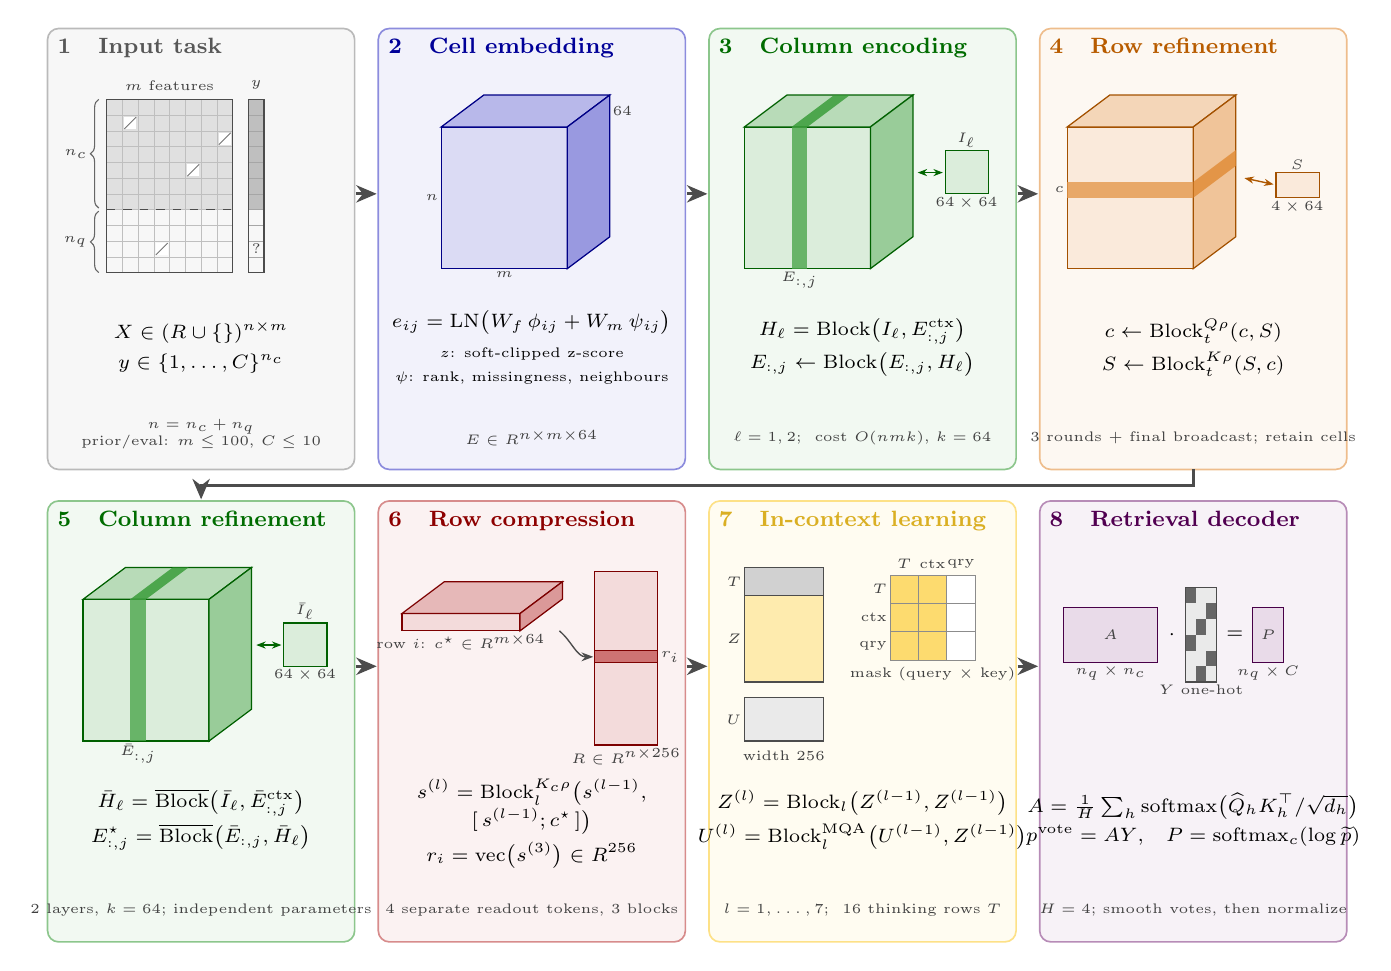
\begin{tikzpicture}[x=1cm, y=1cm]
\tikzset{eqn/.style={font=\fontsize{7.2}{8.8}\selectfont, align=center, inner sep=1pt}}
\def\W{3.9}\def\H{5.6}
\foreach \px/\py/\c in {0/6/cin, 4.2/6/ccell, 8.4/6/ccol, 12.6/6/cref, 0/0/ccol, 4.2/0/crow, 8.4/0/cicl, 12.6/0/cdec}
  \draw[panel=\c] (\px,\py) rectangle ++(\W,\H);
\foreach \a in {3.9, 8.1, 12.3} {
  \draw[bigflow] (\a+0.02,9.5) -- (\a+0.28,9.5);
  \draw[bigflow] (\a+0.02,3.5) -- (\a+0.28,3.5);
}
\draw[bigflow] (14.55,6.0) -- (14.55,5.8) -- (1.95,5.8) -- (1.95,5.62);

% ---------------------------------------------------------------- 1 input
\begin{scope}[shift={(0,6)}]
\node[stitle=cin] at (0.12,5.48) {1\quad Input task};
\fill[black!12] (0.75,3.3) rectangle (2.35,4.7);
\fill[black!3] (0.75,2.5) rectangle (2.35,3.3);
\draw[shift={(0.75,2.5)}, step=0.2, black!25, very thin] (0,0) grid (1.6,2.2);
\draw[black!70, line width=0.45pt] (0.75,2.5) rectangle (2.35,4.7);
\draw[black!70, dashed, line width=0.45pt] (0.75,3.3) -- (2.35,3.3);
% Zero-based cell indices; inset markers are centred on the local grid.
\foreach \col/\row in {1/9, 5/6, 3/1, 7/8} {
  \begin{scope}[shift={({0.75+(\col+0.5)*0.2},{2.5+(\row+0.5)*0.2})}]
    \fill[white] (-0.075,-0.075) rectangle (0.075,0.075);
    \draw[black!55, line width=0.3pt] (-0.075,-0.075) -- (0.075,0.075);
  \end{scope}
}
\fill[black!25] (2.55,3.3) rectangle (2.75,4.7);
\draw[shift={(2.55,2.5)}, step=0.2, black!35, very thin] (0,0) grid (0.2,2.2);
\draw[black!70, line width=0.45pt] (2.55,2.5) rectangle (2.75,4.7);
\node[dim] at (2.65,2.8) {?};
\node[dim] at (1.55,4.88) {$m$ features};
\node[dim] at (2.65,4.88) {$y$};
\draw[decorate, decoration={brace, amplitude=3pt, mirror}, black!60] (0.65,4.7) -- (0.65,3.32) node[midway, left=3pt, dim] {$n_c$};
\draw[decorate, decoration={brace, amplitude=3pt, mirror}, black!60] (0.65,3.28) -- (0.65,2.5) node[midway, left=3pt, dim] {$n_q$};
\node[eqn] at (1.95,1.55) {$X\in(\mathbb{R}\cup\{\varnothing\})^{n\times m}$\\[2pt]$y\in\{1,\dots,C\}^{n_c}$};
\node[dim,align=center] at (1.95,0.45) {$n=n_c+n_q$\\prior/eval: $m\le100$, $C\le10$};
\end{scope}

% ---------------------------------------------------------------- 2 cell embedding
\begin{scope}[shift={(4.2,6)}]
\node[stitle=ccell] at (0.12,5.48) {2\quad Cell embedding};
\tensor{0.8}{2.55}{1.6}{1.8}{0.9}{ccell}
\node[dim, below] at (1.6,2.55) {$m$};
\node[dim, left] at (0.8,3.45) {$n$};
\node[dim] at (3.1,4.55) {$64$};
\node[eqn] at (1.95,1.55) {$e_{ij}=\mathrm{LN}\big(W_f\,\phi_{ij}+W_m\,\psi_{ij}\big)$\\[2pt]
  {\tiny $z$: soft-clipped z-score}\\{\tiny $\psi$: rank, missingness, neighbours}};
\node[dim] at (1.95,0.4) {$E\in\mathbb{R}^{n\times m\times 64}$};
\end{scope}

% ---------------------------------------------------------------- 3 column attention
\begin{scope}[shift={(8.4,6)}]
\node[stitle=ccol] at (0.12,5.48) {3\quad Column encoding};
\tensor{0.45}{2.55}{1.6}{1.8}{0.9}{ccol}
\fill[ccol!70, opacity=0.8] (1.05,2.55) rectangle (1.25,4.35);
\fill[ccol!80, opacity=0.8] (1.05,4.35) -- (1.59,4.755) -- (1.79,4.755) -- (1.25,4.35) -- cycle;
\node[dim, below] at (1.15,2.55) {$E_{:,j}$};
\matrixbox{3.0}{3.5}{0.55}{0.55}{ccol}
\node[dim, above] at (3.27,4.05) {$I_\ell$};
\node[dim, below] at (3.27,3.5) {$64\times 64$};
\draw[{Stealth[length=1.2mm]}-{Stealth[length=1.2mm]}, ccol!80!black, line width=0.5pt] (2.65,3.77) -- (2.97,3.77);
\node[eqn] at (1.95,1.55) {$H_\ell=\mathrm{Block}\big(I_\ell,E^{\mathrm{ctx}}_{:,j}\big)$\\[2pt]$E_{:,j}\leftarrow\mathrm{Block}\big(E_{:,j},H_\ell\big)$};
\node[dim] at (1.95,0.4) {$\ell=1,2$;\ \ cost $O(nmk)$, $k=64$};
\end{scope}

% ---------------------------------------------------------------- 4 row refinement
\begin{scope}[shift={(12.6,6)}]
\node[stitle=cref] at (0.12,5.48) {4\quad Row refinement};
\tensor{0.35}{2.55}{1.6}{1.8}{0.9}{cref}
\fill[cref!70, opacity=0.8] (0.35,3.45) rectangle (1.95,3.65);
\fill[cref!80, opacity=0.8] (1.95,3.45) -- (2.49,3.855) -- (2.49,4.055) -- (1.95,3.65) -- cycle;
\node[dim, left] at (0.35,3.55) {$c$};
\matrixbox{3.0}{3.45}{0.55}{0.32}{cref}
\node[dim, above] at (3.27,3.77) {$S$};
\node[dim, below] at (3.27,3.45) {$4\times 64$};
\draw[{Stealth[length=1.2mm]}-{Stealth[length=1.2mm]}, cref!80!black, line width=0.5pt] (2.6,3.7) -- (2.97,3.62);
\node[eqn] at (1.95,1.55) {$c\leftarrow\mathrm{Block}^{Q\rho}_{t}(c,S)$\\[2pt]$S\leftarrow\mathrm{Block}^{K\rho}_{t}(S,c)$};
\node[dim] at (1.95,0.4) {3 rounds + final broadcast; retain cells};
\end{scope}

% ---------------------------------------------------------------- 5 column refinement
\begin{scope}[shift={(0,0)}]
\node[stitle=ccol] at (0.12,5.48) {5\quad Column refinement};
\tensor{0.45}{2.55}{1.6}{1.8}{0.9}{ccol}
\fill[ccol!70, opacity=0.8] (1.05,2.55) rectangle (1.25,4.35);
\fill[ccol!80, opacity=0.8] (1.05,4.35) -- (1.59,4.755) -- (1.79,4.755) -- (1.25,4.35) -- cycle;
\node[dim, below] at (1.15,2.55) {$\bar E_{:,j}$};
\matrixbox{3.0}{3.5}{0.55}{0.55}{ccol}
\node[dim, above] at (3.27,4.05) {$\bar I_\ell$};
\node[dim, below] at (3.27,3.5) {$64\times 64$};
\draw[{Stealth[length=1.2mm]}-{Stealth[length=1.2mm]}, ccol!80!black, line width=0.5pt] (2.65,3.77) -- (2.97,3.77);
\node[eqn] at (1.95,1.55) {$\bar H_\ell=\overline{\mathrm{Block}}\big(\bar I_\ell,\bar E^{\mathrm{ctx}}_{:,j}\big)$\\[2pt]$E^\star_{:,j}=\overline{\mathrm{Block}}\big(\bar E_{:,j},\bar H_\ell\big)$};
\node[dim] at (1.95,0.4) {2 layers, $k=64$; independent parameters};
\end{scope}

% ---------------------------------------------------------------- 6 row compression
\begin{scope}[shift={(4.2,0)}]
\node[stitle=crow] at (0.12,5.48) {6\quad Row compression};
\tensor{0.3}{3.95}{1.5}{0.22}{0.9}{crow}
\node[dim, below] at (1.05,3.95) {row $i$: $c^\star\in\mathbb{R}^{m\times 64}$};
\matrixbox{2.75}{2.5}{0.8}{2.2}{crow}
\fill[crow!55] (2.75,3.55) rectangle (3.55,3.7);
\draw[crow!75!black, line width=0.45pt] (2.75,3.55) rectangle (3.55,3.7);
\node[dim, below] at (3.15,2.5) {$R\in\mathbb{R}^{n\times 256}$};
\node[dim, right] at (3.55,3.62) {$r_i$};
\draw[flow] (2.3,3.95) to[out=-40, in=180] (2.73,3.62);
\node[eqn] at (1.95,1.5) {$s^{(l)}=\mathrm{Block}^{K_c\rho}_l\big(s^{(l-1)},$\\$[\,s^{(l-1)};c^\star\,]\big)$\\[2pt]$r_i=\mathrm{vec}\big(s^{(3)}\big)\in\mathbb{R}^{256}$};
\node[dim] at (1.95,0.4) {4 separate readout tokens, 3 blocks};
\end{scope}

% ---------------------------------------------------------------- 7 ICL
\begin{scope}[shift={(8.4,0)}]
\node[stitle=cicl] at (0.12,5.48) {7\quad In-context learning};
\fill[black!18] (0.45,4.4) rectangle (1.45,4.75);
\fill[cicl!30] (0.45,3.3) rectangle (1.45,4.4);
\draw[black!70, line width=0.45pt] (0.45,3.3) rectangle (1.45,4.75);
\draw[black!70, line width=0.3pt] (0.45,4.4) -- (1.45,4.4);
\matrixbox{0.45}{2.55}{1.0}{0.55}{cin}
\node[dim, left] at (0.45,4.57) {$T$};
\node[dim, left] at (0.45,3.85) {$Z$};
\node[dim, left] at (0.45,2.82) {$U$};
\node[dim] at (0.95,2.37) {width 256};
\foreach \i in {0,1,2} {
  \foreach \j in {0,1} \filldraw[fill=cicl!55, draw=black!45, line width=0.3pt] (2.3+\j*0.36,4.3-\i*0.36) rectangle ++(0.36,0.36);
  \filldraw[fill=white, draw=black!45, line width=0.3pt] (3.02,4.3-\i*0.36) rectangle ++(0.36,0.36);
}
\foreach \j/\t in {0/$T$, 1/ctx, 2/qry} \node[dim] at (2.48+\j*0.36,4.8) {\t};
\foreach \i/\t in {0/$T$, 1/ctx, 2/qry} \node[dim, anchor=east] at (2.3,4.48-\i*0.36) {\t};
\node[dim] at (2.84,3.4) {mask (query $\times$ key)};
\node[eqn] at (1.95,1.55) {$Z^{(l)}=\mathrm{Block}_l\big(Z^{(l-1)},Z^{(l-1)}\big)$\\[2pt]$U^{(l)}=\mathrm{Block}^{\mathrm{MQA}}_l\big(U^{(l-1)},Z^{(l-1)}\big)$};
\node[dim] at (1.95,0.4) {$l=1,\dots,7$;\ \ 16 thinking rows $T$};
\end{scope}

% ---------------------------------------------------------------- 8 decoder
\begin{scope}[shift={(12.6,0)}]
\node[stitle=cdec] at (0.12,5.48) {8\quad Retrieval decoder};
\matrixbox{0.3}{3.55}{1.2}{0.7}{cdec}
\node[dim] at (0.9,3.9) {$A$};
\node[font=\scriptsize] at (1.68,3.9) {$\cdot$};
\matrixbox{1.85}{3.3}{0.4}{1.2}{cin}
\foreach \r/\c in {0/0, 1/2, 2/1, 3/0, 4/2, 5/1} \fill[black!60] ({1.85+\c*0.1333},{4.5-(\r+1)*0.2}) rectangle ++(0.1333,0.2);
\draw[black!70, line width=0.45pt] (1.85,3.3) rectangle (2.25,4.5);
\node[font=\scriptsize] at (2.48,3.9) {$=$};
\matrixbox{2.7}{3.55}{0.4}{0.7}{cdec}
\node[dim] at (2.9,3.9) {$P$};
\node[dim, below] at (0.9,3.55) {$n_q\times n_c$};
\node[dim, below] at (2.05,3.3) {$Y$ one-hot};
\node[dim, below] at (2.9,3.55) {$n_q\times C$};
\node[eqn] at (1.95,1.55) {$A=\frac{1}{H}\sum_h\mathrm{softmax}\big(\widehat Q_hK_h^\top/\sqrt{d_h}\big)$\\[2pt]$p^{\mathrm{vote}}=AY$,\quad $P=\mathrm{softmax}_c(\log\widetilde p)$};
\node[dim] at (1.95,0.4) {$H=4$; smooth votes, then normalize};
\end{scope}

\end{tikzpicture}
}
\caption{B4 from the input table through seven operators. Both column stages gather from labelled context
cells and broadcast to context and query cells. Row refinement exchanges information through
temporary summaries while retaining the cells; row compression uses a separate set of summaries.
The second column stage is an explicit step between refinement and compression. Tensor shapes,
attention directions and the context/query mask are shown for one task.}
\label{fig:arch}
\end{figure}

\begin{figure}[tbp]
\centering
\resizebox{\linewidth}{!}{% Architecture of LightPFN (variant B4), details: cell embedding, column ISAB and row refinement on
% the first row, ICL block and decoder on the second. Portrait, about 13.7 cm wide before scaling.
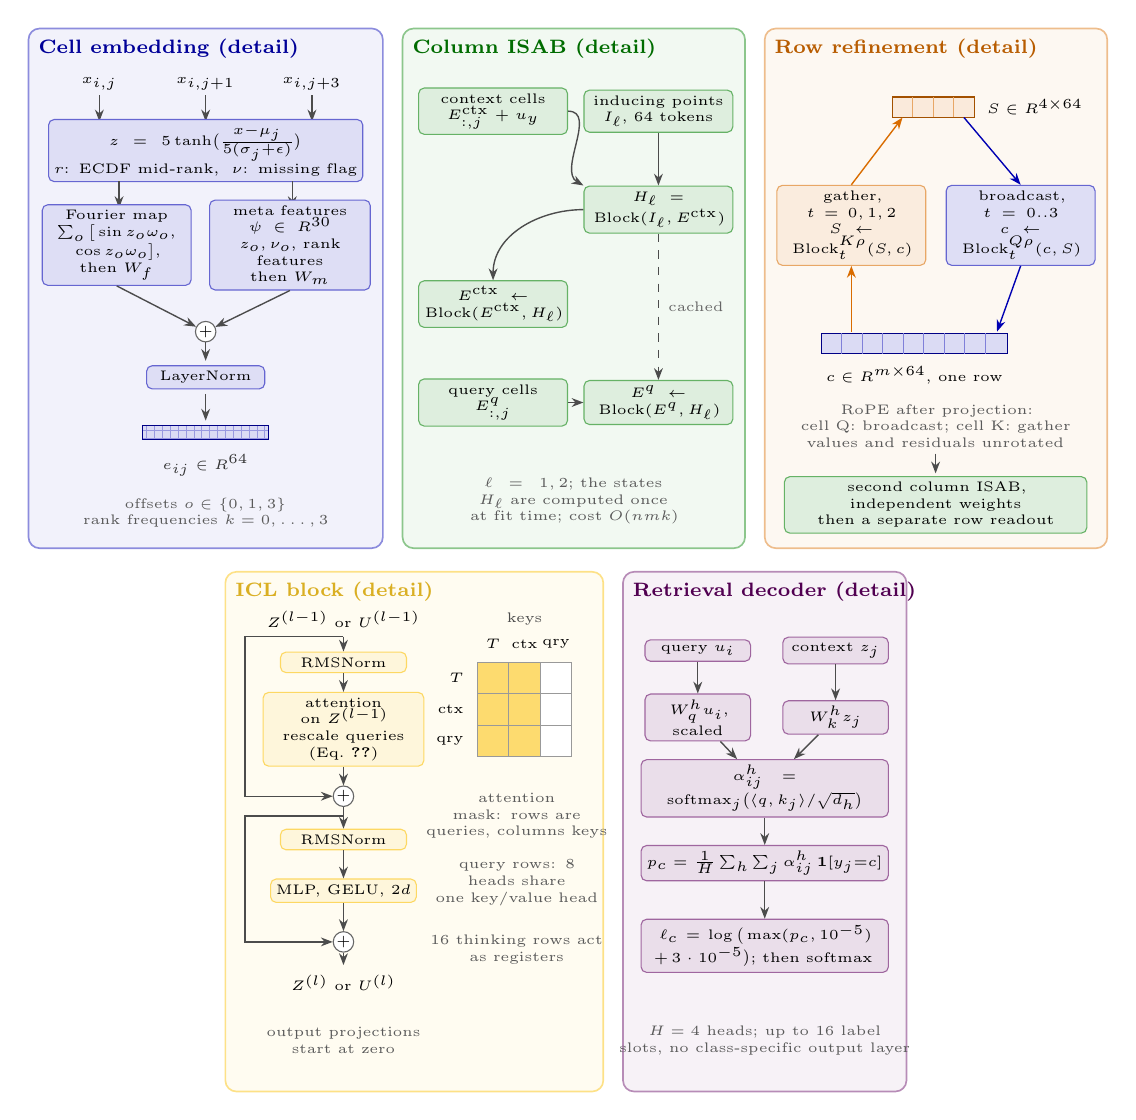
\begin{tikzpicture}[x=1cm, y=1cm]
\def\db{0}\def\dt{6.6}
\draw[panel=ccell] (0,\db)     rectangle (4.5,\dt);
\draw[panel=ccol]  (4.75,\db)  rectangle (9.1,\dt);
\draw[panel=cref]  (9.35,\db)  rectangle (13.7,\dt);

% cell embedding detail
\node[ptitle=ccell] at (0.12,6.48) {Cell embedding (detail)};
\foreach \x/\t in {0.9/{$x_{i,j}$}, 2.25/{$x_{i,j+1}$}, 3.6/{$x_{i,j+3}$}} {
  \node[font=\tiny] at (\x,5.9) {\t};
  \draw[flow] (\x,5.75) -- (\x,5.42);
}
\node[sbox=ccell, text width=3.85cm] at (2.25,5.05)
  {$z=5\tanh\!\big(\tfrac{x-\mu_j}{5(\sigma_j+\epsilon)}\big)$\\$r$: ECDF mid-rank,\ \ $\nu$: missing flag};
\draw[flow] (1.15,4.66) -- (1.15,4.32);
\draw[flow] (3.35,4.66) -- (3.35,4.32);
\node[sbox=ccell, text width=1.75cm] (fo) at (1.12,3.85)
  {Fourier map\\$\sum_o\big[\sin z_o\omega_o,$\\$\cos z_o\omega_o\big]$, then $W_f$};
\node[sbox=ccell, text width=1.9cm] (me) at (3.32,3.85)
  {meta features $\psi\in\mathbb{R}^{30}$\\$z_o,\nu_o$, rank features\\then $W_m$};
\node[plus] (p1) at (2.25,2.75) {$+$};
\draw[flow] (fo.south) -- (p1);
\draw[flow] (me.south) -- (p1);
\draw[flow] (p1) -- (2.25,2.38);
\node[sbox=ccell, minimum width=1.5cm] at (2.25,2.17) {LayerNorm};
\draw[flow] (2.25,1.96) -- (2.25,1.62);
\matrixbox{1.45}{1.38}{1.6}{0.18}{ccell}
\draw[step=0.1, ccell!40, very thin] (1.45,1.38) grid (3.05,1.56);
\draw[ccell!75!black, line width=0.45pt] (1.45,1.38) rectangle (3.05,1.56);
\node[shapelabel] at (2.25,1.05) {$e_{ij}\in\mathbb{R}^{64}$};
\node[note] at (2.25,0.45) {offsets $o\in\{0,1,3\}$\\rank frequencies $k=0,\dots,3$};

% column ISAB detail
\node[ptitle=ccol] at (4.87,6.48) {Column ISAB (detail)};
\node[sbox=ccol, text width=1.75cm] (ctx) at (5.9,5.55) {context cells\\$E^{\mathrm{ctx}}_{:,j}+u_{y}$};
\node[sbox=ccol, text width=1.75cm] (ind) at (8.0,5.55) {inducing points\\$I_\ell$, 64 tokens};
\node[sbox=ccol, text width=1.75cm] (H) at (8.0,4.3) {$H_\ell=$\\$\mathrm{Block}(I_\ell,E^{\mathrm{ctx}})$};
\draw[flow] (ind) -- (H);
\draw[flow] (ctx.east) to[out=0, in=150] (H.north west);
\node[sbox=ccol, text width=1.75cm] (C2) at (5.9,3.1) {$E^{\mathrm{ctx}}\leftarrow$\\$\mathrm{Block}(E^{\mathrm{ctx}},H_\ell)$};
\draw[flow] (H.west) to[out=180, in=90] (C2.north);
\node[sbox=ccol, text width=1.75cm] (qc) at (5.9,1.85) {query cells\\$E^{q}_{:,j}$};
\node[sbox=ccol, text width=1.75cm] (Q2) at (8.0,1.85) {$E^{q}\leftarrow$\\$\mathrm{Block}(E^{q},H_\ell)$};
\draw[flow] (qc) -- (Q2);
\draw[flow, dashed] (H.south) -- node[right, font=\tiny, text=black!60] {cached} (Q2.north);
\node[note, text width=4.0cm] at (6.92,0.6) {$\ell=1,2$; the states $H_\ell$ are computed once\\at fit time; cost $O(nmk)$};

% row refinement detail
\node[ptitle=cref] at (9.47,6.48) {Row refinement (detail)};
\matrixbox{10.97}{5.47}{1.04}{0.26}{cref}
\foreach \x in {11.23,11.49,11.75} \draw[cref!60, line width=0.3pt] (\x,5.47) -- (\x,5.73);
\node[font=\tiny, anchor=west] at (12.05,5.6) {$S\in\mathbb{R}^{4\times 64}$};
\matrixbox{10.07}{2.47}{2.36}{0.26}{ccell}
\foreach \x in {10.33,10.59,10.85,11.11,11.37,11.63,11.89,12.15} \draw[ccell!50, line width=0.3pt] (\x,2.47) -- (\x,2.73);
\node[font=\tiny, anchor=north] at (11.25,2.43) {$c\in\mathbb{R}^{m\times 64}$, one row};
\node[sbox=cref, text width=1.75cm] (ga) at (10.45,4.1) {gather, $t=0,1,2$\\$S\leftarrow\mathrm{Block}^{K\rho}_t(S,c)$};
\node[sbox=ccell, text width=1.75cm] (bc) at (12.6,4.1) {broadcast, $t=0..3$\\$c\leftarrow\mathrm{Block}^{Q\rho}_t(c,S)$};
\draw[flow, cref] (10.45,2.75) -- (ga.south);
\draw[flow, cref] (ga.north) -- (11.1,5.47);
\draw[flow, ccell] (11.88,5.47) -- (bc.north);
\draw[flow, ccell] (bc.south) -- (12.3,2.75);
\node[note, text width=4.1cm] at (11.52,1.55) {RoPE after projection:\\cell Q: broadcast; cell K: gather\\values and residuals unrotated};
\draw[flow] (11.52,1.2) -- (11.52,0.95);
\node[sbox=ccol, text width=3.7cm] at (11.52,0.55) {second column ISAB, independent weights\\then a separate row readout};

% second row
\begin{scope}[xshift=-11.45cm, yshift=-6.9cm]
\draw[panel=cicl]  (13.95,\db) rectangle (18.75,\dt);
\draw[panel=cdec]  (19.0,\db)  rectangle (22.6,\dt);

% ICL block detail
\node[ptitle=cicl] at (14.07,6.48) {ICL block (detail)};
\node[font=\tiny] (in) at (15.45,6.0) {$Z^{(l-1)}$ or $U^{(l-1)}$};
\node[sbox=cicl, minimum width=1.6cm] (n1) at (15.45,5.45) {RMSNorm};
\node[sbox=cicl, text width=1.9cm] (at) at (15.45,4.6) {attention on $Z^{(l-1)}$\\rescale queries\\(Eq.~\ref{eq:query-scaling})};
\node[plus] (a1) at (15.45,3.75) {$+$};
\node[sbox=cicl, minimum width=1.6cm] (n2) at (15.45,3.2) {RMSNorm};
\node[sbox=cicl, minimum width=1.6cm] (ml) at (15.45,2.55) {MLP, GELU, $2d$};
\node[plus] (a2) at (15.45,1.9) {$+$};
\node[font=\tiny] (out) at (15.45,1.38) {$Z^{(l)}$ or $U^{(l)}$};
\draw[flow] (in) -- (n1); \draw[flow] (n1) -- (at); \draw[flow] (at) -- (a1);
\draw[flow] (a1) -- (n2); \draw[flow] (n2) -- (ml); \draw[flow] (ml) -- (a2); \draw[flow] (a2) -- (out);
\draw[flow] (15.45,5.78) -- (14.2,5.78) -- (14.2,3.75) -- (a1);
\draw[flow] (15.45,3.5) -- (14.2,3.5) -- (14.2,1.9) -- (a2);
\node[note] at (15.45,0.65) {output projections\\start at zero};
% attention mask: rows are queries, columns are keys
\node[font=\tiny, text=black!70] at (17.75,6.0) {keys};
\foreach \j/\t in {0/$T$, 1/ctx, 2/qry} \node[font=\tiny] at (17.35+\j*0.4,5.68) {\t};
\foreach \i/\t in {0/$T$, 1/ctx, 2/qry} \node[font=\tiny, anchor=east] at (17.1,5.25-\i*0.4) {\t};
\foreach \i in {0,1,2} {
  \foreach \j in {0,1} \filldraw[fill=cicl!55, draw=black!40, line width=0.3pt] (17.15+\j*0.4,5.05-\i*0.4) rectangle ++(0.4,0.4);
  \filldraw[fill=white, draw=black!40, line width=0.3pt] (17.95,5.05-\i*0.4) rectangle ++(0.4,0.4);
}
\node[note, text width=2.3cm] at (17.65,3.5) {attention mask: rows are\\queries, columns keys};
\node[note, text width=2.3cm] at (17.65,2.65) {query rows: 8 heads share\\one key/value head};
\node[note, text width=2.3cm] at (17.65,1.8) {16 thinking rows act\\as registers};

% decoder detail
\node[ptitle=cdec] at (19.12,6.48) {Retrieval decoder (detail)};
\node[sbox=cdec, text width=1.2cm] (ui) at (19.95,5.6) {query $u_i$};
\node[sbox=cdec, text width=1.2cm] (zj) at (21.7,5.6) {context $z_j$};
\node[sbox=cdec, text width=1.2cm] (qh) at (19.95,4.75) {$W_q^h u_i$, scaled};
\node[sbox=cdec, text width=1.2cm] (kh) at (21.7,4.75) {$W_k^h z_j$};
\draw[flow] (ui) -- (qh); \draw[flow] (zj) -- (kh);
\node[sbox=cdec, text width=3.0cm] (al) at (20.8,3.85) {$\alpha^h_{ij}=\mathrm{softmax}_j\big(\langle q,k_j\rangle/\sqrt{d_h}\big)$};
\draw[flow] (qh) -- (al); \draw[flow] (kh) -- (al);
\node[sbox=cdec, text width=3.0cm] (pp) at (20.8,2.9) {$p_c=\frac{1}{H}\sum_h\sum_j\alpha^h_{ij}\,\mathbf{1}[y_j{=}c]$};
\draw[flow] (al) -- (pp);
\node[sbox=cdec, text width=3.0cm] (lg) at (20.8,1.85) {$\ell_c=\log\big(\max(p_c,10^{-5})$\\$+\,3\cdot10^{-5}\big)$; then softmax};
\draw[flow] (pp) -- (lg);
\node[note] at (20.8,0.65) {$H=4$ heads; up to 16 label\\slots, no class-specific output layer};
\end{scope}
\end{tikzpicture}
}
\caption{Cell embedding, column ISAB, row refinement, an ICL block and label retrieval. The dashed column arrow
denotes cached memory. Rotary positions act on projected cell queries in
broadcast and on projected cell keys in gather and pooling. Cell values and residual states are
unrotated. The column pattern is used twice with independent parameters.}
\label{fig:arch-details}
\end{figure}

\subsection{Attention block}
Attention modules use the same pre-norm residual block structure, with their own parameters.
Let $X\in\R^{L_q\times d}$ be the query sequence and $Y\in\R^{L_k\times d}$ the source sequence.
Each head projects separately normalized states into queries, keys and values, using the
output-by-input weight convention of the implementation:
\begin{equation}
\begin{aligned}
Q_h&=\RMS_Q(X)W_{Q,h}^{\top},\\
K_h&=\RMS_{KV}(Y)W_{K,h}^{\top},\qquad
V_h=\RMS_{KV}(Y)W_{V,h}^{\top}.
\end{aligned}
\end{equation}
\begin{align}
\widetilde X&=X+\operatorname{Concat}_h
 \left[\operatorname{softmax}\!\left(\frac{\widehat Q_h\widehat K_h^\top}{\sqrt{d_h}}+M\right)V_h\right]W_O^{\top},\\
\Block(X,Y)&=\widetilde X+\mathrm{GELU}\big(\RMS_{FF}(\widetilde X)W_1^{\top}\big)W_2^{\top}.
\label{eq:block}
\end{align}
Here $M$ is an additive mask with zero on allowed keys and $-\infty$ on excluded keys, and
$W_1\in\R^{2d\times d}$. Ordinarily $\widehat Q_h=Q_h$ and $\widehat K_h=K_h$; positional rotation
or query scaling modifies these projections where specified below. We write $\Block^{Q\rho}$
when rotary positions act on cell queries, $\Block^{K\rho}$ when they act on cell keys, and
$\Block^{K_c\rho}$ when only the cell subset of a mixed source is rotated. The values and residual
state are unchanged by these positional operations. Output projections $W_O$ and $W_2$ start at
zero, so each block is the identity at initialization. Cached source keys and values are projected
once and reused for subsequent queries.

\subsection{Cell embedding}
Statistics are computed on the context rows of each column $j$, ignoring missing values: the mean
$\mu_j$, the standard deviation $\sigma_j$ and the sorted values. A cell is described by a
soft-clipped z-score, a mid-rank under the empirical CDF of the context, and a missingness flag:
\begin{equation}
z_{ij}=5\tanh\!\Big(\frac{x_{ij}-\mu_j}{5(\sigma_j+\epsilon)}\Big),\qquad
r_{ij}=\frac{\#\{x_{lj}<x_{ij}\}+\#\{x_{lj}\le x_{ij}\}}{2\,N_j},\qquad
\nu_{ij}=\mathbf{1}[x_{ij}\text{ missing}],
\end{equation}
where counts run over the $N_j$ observed context values; missing cells get $z=0$ and $r=1/2$.
The standard deviation uses denominator $\max(N_j-1,1)$; constant columns receive $z=0$, and
entirely unobserved columns receive $r=1/2$. The mean and standard deviation are conventional
sample statistics: soft clipping bounds the normalized values but does not make these estimators robust.
Each cell also sees two neighbouring columns through circular offsets $o\in\{0,1,3\}$, which gives
the embedding a cheap view of local feature pairs. With learned frequencies
$\omega_o\in\R^{16}$, the value part is a Fourier feature map \cite{tancik2020}, and the rank part
uses fixed dyadic frequencies:
\begin{align}
e^{\mathrm{val}}_{ij}&=W_f\sum_{o}\big[\sin(z_{i,j+o}\,\omega_o),\ \cos(z_{i,j+o}\,\omega_o)\big],\\
e^{\mathrm{meta}}_{ij}&=W_m\psi_{ij},\qquad
\psi_{ij}=\big[(z_{i,j+o})_o;\ (\nu_{i,j+o})_o;\
 (\sin(2^k\pi r_{i,j+o}))_{o,k};\
 (\cos(2^k\pi r_{i,j+o}))_{o,k}\big]\in\R^{30},\\
e_{ij}&=\LN\big(e^{\mathrm{val}}_{ij}+e^{\mathrm{meta}}_{ij}\big)\in\R^{64}.
\end{align}
Here $o\in\{0,1,3\}$ and $k=0,\dots,3$. Offsets wrap modulo the true feature count; padding is excluded from feature attention. All
statistics are fitted to the context and reused for queries. Categorical columns enter as ordinal codes of
their categories, through the same embedding as numeric columns; the network has no categorical-specific
encoding (Section~\ref{sec:categorical}).

\subsection{Column encoding}
The first column operator $\mathcal{C}_1$ uses induced set attention blocks (ISAB) \cite{lee2019}.
It acts independently on the row sequence of each column, with parameters shared across columns.
Context cells start from $E^{(0)}_{ij}+u^{(1)}_{y_i}$; query cells start from $E^{(0)}_{ij}$.
Label embeddings have orthonormal initialization and are subsequently learned without an
orthogonality constraint. With $k=64$ learned inducing tokens $I_\ell$ per layer, the updates are
\begin{equation}
H_{\ell j}=\Block^{\mathrm{ind}}_\ell(I_\ell,E^{\mathrm{ctx}}_{:,j}),\qquad
E^a_{:,j}\leftarrow\Block^{\mathrm{cell}}_\ell(E^a_{:,j},H_{\ell j}),
\quad a\in\{\mathrm{ctx},q\},\quad \ell=1,2.
\end{equation}
The gather and broadcast blocks have separate parameters; the broadcast weights are shared between
context and query cells. Query cells never contribute to $H_{\ell j}$. For prediction, the projected
keys and values of each $H_{\ell j}$ are cached. This makes the encoding sensitive to the labelled
column distribution, with attention cost $O(nmk)$ at fixed depth and width.

\subsection{Row refinement}
The operator $\mathcal{F}$ exchanges information across the feature axis while retaining all cell
states. It follows the summary-mediated refinement of Causilo \cite{causilo}. Each row starts with
its cells $c^{(0)}\in\R^{m\times64}$ and $K=4$ learned temporary tokens
$S^{(0)}\in\R^{K\times64}$, initialized identically across rows. For $t=0,\dots,R-1$,
\begin{align}
c^{(t+1)}&=\Block_t^{\mathrm{bc},Q\rho}\big(c^{(t)},S^{(t)}\big),\\
S^{(t+1)}&=\Block_t^{\mathrm{ga},K\rho}\big(S^{(t)},c^{(t+1)}\big),
\end{align}
followed by a final broadcast
\begin{equation}
\bar c=\Block_R^{\mathrm{bc},Q\rho}\big(c^{(R)},S^{(R)}\big).
\end{equation}
With $R=3$, there are four broadcast and three gather blocks, all independently parameterized.
Rotary position embedding \cite{su2024} acts on projected cell queries during broadcast and
projected cell keys during gather. Only after the first gather do the temporary tokens carry
row-specific evidence from other features. The final broadcast returns this evidence to the cells;
the temporary tokens are then discarded. The attention cost is $O((2R+1)nmK)$, linear in $m$
for fixed $R$ and $K$, compared with $O(nm^2)$ for the baseline's full row self-attention.

\subsection{Column refinement}
The operator $\mathcal{C}_2$ applies the same two-layer induced attention pattern as
$\mathcal{C}_1$, with independent inducing tokens, projections, feed-forward blocks and label
embeddings $u^{(2)}_y$. Its context input is $\bar E^{\mathrm{ctx}}_{ij}+u^{(2)}_{y_i}$ and its
query input is $\bar E^q_{ij}$. The context-only gather now reads cells that already encode
within-row feature interactions. The broadcast compares each such cell with this enriched column
memory before any feature information is pooled away. The second stage has its own cached keys
and values, and the same $O(nmk)$ attention cost as the first.

\subsection{Row compression}
The pooling operator $\mathcal{P}$ uses $K_p=4$ learned readout tokens
$s^{(0)}\in\R^{K_p\times64}$, separate from the temporary tokens of $\mathcal{F}$. For each row,
three attention blocks update these readout tokens while holding the refined cells $c^\star$ fixed:
\begin{equation}
s^{(l)}=\Block_l^{K_c\rho}\big(s^{(l-1)},[\,s^{(l-1)};c^\star\,]\big),\qquad
r_i=\mathrm{vec}\big(s^{(3)}\big)\in\R^{256}.
\end{equation}
Only the cell keys receive rotary positions; summary keys and all values remain unrotated.
The attention cost is $O(nK_p(m+K_p))$ at fixed depth. This operation removes the feature axis
and supplies a fixed-width representation to ICL. B3 ablated this pooling in place of full row
self-attention: its accuracy differences from A0 were inconclusive, and its training time was 70\%
of A0's. This supports it as an efficient readout, without establishing statistical equivalence.

\subsection{In-context learning stage}
Context rows receive a row-level label embedding $v_{y_i}\in\R^{256}$ and are preceded by 16 learned
thinking rows $T$, which act as registers \cite{darcet2024}. With $Z^{(0)}=[\,T;\ R_{\mathrm{ctx}}+V_{y}\,]$
and query rows $U^{(0)}=R_{q}$, each of the $L=7$ blocks computes
\begin{equation}
Z^{(l)}=\Block_l\big(Z^{(l-1)},Z^{(l-1)}\big),\qquad
U^{(l)}=\Block_l^{\mathrm{MQA}}\big(U^{(l-1)},Z^{(l-1)}\big).
\end{equation}
Context and query updates share block parameters, but use different key/value head patterns.
Context rows use eight-head self-attention; query rows attend to the context and thinking rows
using multi-query attention \cite{shazeer2019}, with all eight query heads reading the first
key/value head. Query rows never attend to each other, and the context never reads them. The
prediction cache therefore stores one eighth of the full per-layer ICL keys and values; this
cache ratio does not imply an eightfold reduction in total inference cost. To adapt attention
sharpness to the number of source keys $N$, projected queries are rescaled by
\begin{equation}
q\leftarrow q\odot\beta(\log\max(N,2))\odot\big(1+\tanh\varphi(q)\big),
\label{eq:query-scaling}
\end{equation}
where $\beta$ and $\varphi$ are learned MLPs initialized to make scaling the identity, and
$N=n_c+16$ in ICL. A final RMS normalization is applied to context and query row states.

\subsection{Retrieval decoder}
The readout is an attention-weighted vote of the context labels. With $H=4$ heads,
queries from the final query states $u_i$ and keys from the final context states $z_j$,
\begin{equation}
\begin{aligned}
\alpha^{h}_{ij}&=\operatorname{softmax}_j\Big(\frac{\langle \widehat q_i^h,\ W_k^h z_j\rangle}{\sqrt{d_h}}\Big),\\
p^{\mathrm{vote}}_{ic}&=\frac{1}{H}\sum_{h=1}^{H}\sum_{j\in\Dc}
\alpha^{h}_{ij}\,\mathbf{1}[y_j=c].
\end{aligned}
\end{equation}
Here $\widehat q_i^h$ is $W_q^h u_i$ after key-count scaling with $N=n_c$; the decoder has its
own scaling parameters. One-hot context labels supply the values, and the thinking rows are
excluded. The decoder returns logits
\begin{equation}
\begin{aligned}
\widetilde p_{ic}&=\max(p^{\mathrm{vote}}_{ic},10^{-5})+3\cdot10^{-5},
\qquad \ell_{ic}=\log\widetilde p_{ic},\\
q_\theta(y=c\mid x_i,\Dc)&=\operatorname{softmax}_c(\ell_i)_c.
\end{aligned}
\end{equation}
The smoothing bounds the loss of a confident mistake; the final softmax renormalizes the smoothed
votes. No learned output vector is needed per class. Although the attention value width is 64,
the complete model's label-embedding interface supports at most 16 classes; the training prior
contains 2--10 classes, so support for 11--16 is a capacity limit rather than an evaluated guarantee.

\paragraph{Label slots.} The model has 16 label slots. During training the $C$ classes of every task
are mapped to a random injective assignment of slots, exposing all slot embeddings to training
and discouraging dependence on a fixed class index. Random slot assignment does not impose exact
class-permutation equivariance on the learned embeddings.

\subsection{Symmetries and attention cost}
In exact arithmetic, permuting context rows together with their labels leaves query predictions
unchanged: column summaries and ICL have no row-position encoding, and retrieval sums over the
permuted context. Permuting query rows permutes their outputs, and a query's prediction does not
depend on other queries. Finite-precision reductions can introduce small numerical differences.
Feature-order invariance is not imposed: both circular feature grouping and rotary positions depend
on column order. Random feature permutations during training and permutation ensembles encourage
robustness but do not establish an exact symmetry.

At fixed depths and widths, the attention interactions in the two column stages, row refinement,
row pooling and ICL scale as
\begin{equation}
O\!\left(nmk+(2R+1)nmK+nK_p(m+K_p)
 +(n_c+16)^2+n_q(n_c+16)\right).
\end{equation}
Retrieval adds $O(n_qn_c)$. These expressions describe attention interactions, not wall-clock time:
projections and feed-forward blocks remain, and sorting context values for ECDF preprocessing costs
$O(mn_c\log n_c)$, followed by $O(nm\log n_c)$ rank lookups. B4 is linear in the feature count
for fixed $k,R,K,K_p$, but still quadratic
in the context length. Section~\ref{sec:cost} reports the measured CPU trade-off.

\subsection{Parameter budget and inference}
Table~\ref{tab:params} lists the parameter counts. B4 adds 372,032 parameters in the refinement
loop and the second column stage and removes one ICL block of 546,016 parameters, for a total of
4,603,088. At inference, fitting encodes the context once and stores the column statistics, the
inducing-point states of both column stages, the ICL keys and values and the decoder keys; prediction
then processes query rows in independent chunks. An ensemble of $E$
estimators averages the probabilities obtained under random permutations of feature order and class
slots. By default, above 20,000 training rows, each estimator uses a stratified context subsample that
retains every class. The full-context experiments in Section~\ref{sec:large} override this limit.
Section~\ref{sec:inference} describes a faster implementation of these steps that computes the
same predictions up to floating-point rounding.

\begin{table}[t]
\centering
\small
\begin{tabular}{lrr}
\toprule
Component & A0 & B4 \\
\midrule
Cell embedding & 4,144 & 4,144 \\
Column encoding & 141,056 & 141,056 \\
Row refinement ($R=3$) & 0 & 230,976 \\
Column refinement & 0 & 141,056 \\
Row encoder / compression & 99,136 & 99,136 \\
ICL, including labels, registers and final norm & 4,376,128 & 3,830,560 \\
Retrieval decoder & 156,160 & 156,160 \\
\midrule
Total trainable parameters & 4,777,072 & 4,603,088 \\
\bottomrule
\end{tabular}
\caption{Trainable parameter counts. Each ICL block contains 546,016 parameters. The 372,032
parameters of row and column refinement are funded by reducing ICL depth from eight to seven.
The baseline row encoder and B4 pooling have the same parameter count but different attention
patterns. B4 is 173,984 parameters smaller than A0.}
\label{tab:params}
\end{table}

\section{Synthetic priors}
\label{sec:prior}

\subsection{Task geometry}
Tasks are generated in groups of eight that share their shape, which keeps padding low during
training. The number of rows is log-uniform, $n\sim\mathrm{LogU}(256,2048)$, and the context
fraction is uniform in $[0.3,0.9]$. The number of features follows the ratio $m/n$, drawn
log-uniformly within one of three bands, $[0.01,0.06]$ with probability 0.7, $[0.06,0.15]$ with
probability 0.2 and $[0.15,0.5]$ with probability 0.1, then rounded and clipped to $[2,100]$. A task
is binary with probability $p_{\mathrm{bin}}$ and otherwise has $C\sim\mathcal{U}\{3,\dots,10\}$
classes. Half of the tasks are resampled to an imbalanced class distribution, with a binary
minority share drawn from $\mathrm{LogU}(0.01,0.5)$ and multiclass proportions from a Dirichlet
distribution. Every random draw is seeded by its coordinates (prior, shard, group, task, phase) through a
hierarchical seed sequence, so shards are byte-identical for any number of worker processes.

\subsection{Graph prior}
The graph prior reproduces the structural causal model of TabICLv2 \cite{tabiclv2} deterministically.
A random directed acyclic graph is sampled; each node applies a random function to its parents,
chosen among MLPs, random oblivious trees, discretizations, linear and quadratic maps, Gaussian
processes with product kernels and products, with sum, product, max or log-sum-exp aggregation and
Kumaraswamy warping; some nodes become categorical. Features and the target are read from selected
nodes. Each draft task passes an out-of-bag filter based on ExtraTrees \cite{geurts2006}, which
rejects tasks whose labels cannot be predicted at all. Version 3 uses $p_{\mathrm{bin}}=0.55$.
Version 4 keeps heavy tails in most tasks, quantizes some numeric columns into categorical codes
with cardinality $\mathrm{LogU}(16,256)$ and Zipf frequencies, raises $p_{\mathrm{bin}}$ to 0.78,
splits numeric targets at quantiles for part of the multiclass tasks and reads the target from the
final node in 90\% of the drafts.

\subsection{Rule prior}
The rule prior draws features from graph v4 and assigns labels with a known oracle over one to four
observed driver columns. Its families and probabilities are XOR (25\%), parity (20\%), shallow trees
(20\%), lookup tables (10\%), products (10\%), AND (7.5\%) and OR (7.5\%). For binary XOR and parity,
the drivers are resampled independently within the partitions of their marginal distributions, with
source thresholds $\tau_k$ at quantiles between 30\% and 70\%, and the label is
\begin{equation}
y=\bigoplus_{k=1}^{K}\mathbf{1}\big[x_{d_k}>\tau_k\big].
\end{equation}
Since the factorial cells are balanced, $P(y=1\mid x_{d_k})=1/2$ for every single driver: the
signal lives entirely in the interaction. For $C$ classes, each driver is mapped to a symbol
$s_k\in\{0,\dots,C-1\}$ with uniform frequencies and $y=\big(\sum_k s_k\big)\bmod C$, a Latin-square
construction with the same property (Figure~\ref{fig:rules}). Tree, lookup, product, AND and OR tasks receive, in a quarter
of the cases, a mixture with the logits of the underlying graph,
\begin{equation}
\ell=a\,\ell_{\mathrm{rule}}+b\,\ell_{\mathrm{graph}},\qquad a\sim\mathcal{U}[0.75,1.5],\ b\sim\mathcal{U}[0,0.5],
\end{equation}
followed by a softmax at temperature 0.125. Label noise between 0\% and 15\% is added, and a gate
requires at least two rows per class and an agreement of at least 70\% between the oracle and the
noisy test labels. No fitted classifier is used to filter rule tasks.

\begin{figure}[tbp]
\centering
% Rule prior: interaction-only constructions (binary XOR and a Latin square for C = 3).
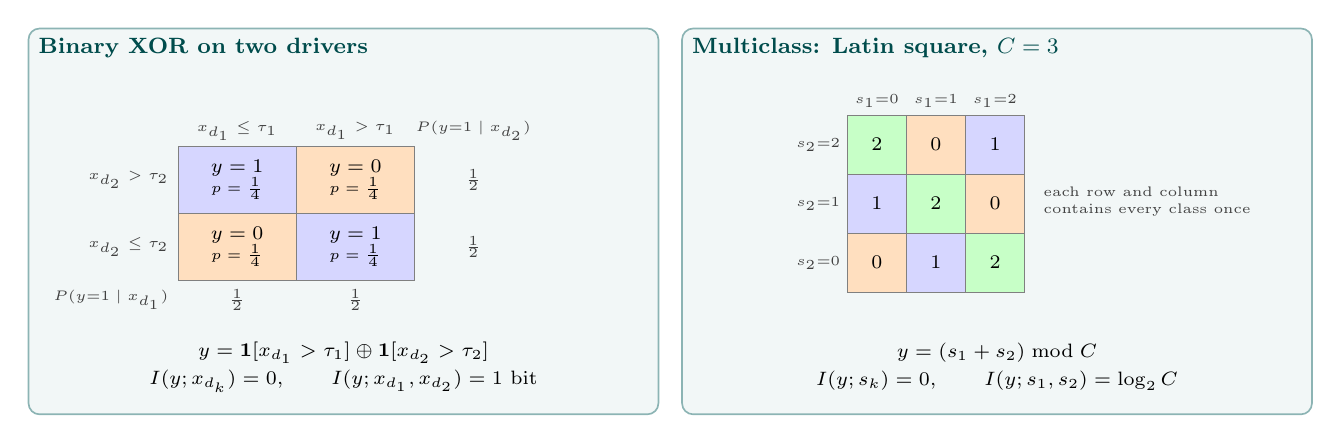
\begin{tikzpicture}[x=1cm, y=1cm]
\draw[panel=cdata] (0,0) rectangle (8.0,4.9);
\draw[panel=cdata] (8.3,0) rectangle (16.3,4.9);

% binary XOR: 2 x 2 table of the balanced factorial cells with conditional probabilities
\node[stitle=cdata] at (0.12,4.78) {Binary XOR on two drivers};
\def\ox{1.9}\def\oy{1.7}\def\cw{1.5}\def\ch{0.85}
\foreach \i/\j/\v in {0/0/0, 1/0/1, 0/1/1, 1/1/0} {
  \ifnum\v=0 \def\col{orange!25}\else \def\col{blue!16}\fi
  \filldraw[fill=\col, draw=black!50, line width=0.4pt] (\ox+\i*\cw,\oy+\j*\ch) rectangle ++(\cw,\ch);
  \node[font=\scriptsize, align=center] at (\ox+\i*\cw+0.5*\cw,\oy+\j*\ch+0.5*\ch) {$y=\v$\\[-1pt]{\tiny $p=\tfrac14$}};
}
\node[dim] at (\ox+0.5*\cw,\oy+2*\ch+0.2) {$x_{d_1}\le\tau_1$};
\node[dim] at (\ox+1.5*\cw,\oy+2*\ch+0.2) {$x_{d_1}>\tau_1$};
\node[dim, anchor=east] at (\ox-0.08,\oy+1.5*\ch) {$x_{d_2}>\tau_2$};
\node[dim, anchor=east] at (\ox-0.08,\oy+0.5*\ch) {$x_{d_2}\le\tau_2$};
\node[dim] at (\ox+2*\cw+0.75,\oy+2*\ch+0.2) {$P(y{=}1\mid x_{d_2})$};
\foreach \j in {0,1} \node[dim] at (\ox+2*\cw+0.75,\oy+\j*\ch+0.5*\ch) {$\tfrac12$};
\node[dim, anchor=east] at (\ox-0.08,\oy-0.25) {$P(y{=}1\mid x_{d_1})$};
\foreach \i in {0,1} \node[dim] at (\ox+\i*\cw+0.5*\cw,\oy-0.25) {$\tfrac12$};
\node[font=\scriptsize, align=center] at (4.0,0.6)
  {$y=\mathbf{1}[x_{d_1}>\tau_1]\oplus\mathbf{1}[x_{d_2}>\tau_2]$\\[2pt]
   $I(y;x_{d_k})=0,\qquad I(y;x_{d_1},x_{d_2})=1$ bit};

% Latin square for C = 3
\node[stitle=cdata] at (8.42,4.78) {Multiclass: Latin square, $C=3$};
\def\lx{10.4}\def\ly{1.55}\def\s{0.75}
\foreach \a in {0,1,2} \foreach \b in {0,1,2} {
  \pgfmathtruncatemacro{\c}{mod(\a+\b,3)}
  \ifcase\c \def\col{orange!25}\or \def\col{blue!16}\or \def\col{green!22}\fi
  \filldraw[fill=\col, draw=black!50, line width=0.4pt] (\lx+\a*\s,\ly+\b*\s) rectangle ++(\s,\s);
  \node[font=\scriptsize] at (\lx+\a*\s+0.5*\s,\ly+\b*\s+0.5*\s) {$\c$};
}
\foreach \a in {0,1,2} {
  \node[dim] at (\lx+\a*\s+0.5*\s,\ly+3*\s+0.18) {$s_1{=}\a$};
  \node[dim, anchor=east] at (\lx-0.05,\ly+\a*\s+0.5*\s) {$s_2{=}\a$};
}
\node[dim, anchor=west, align=left] at (12.85,2.7) {each row and column\\contains every class once};
\node[font=\scriptsize, align=center] at (12.3,0.6)
  {$y=(s_1+s_2)\bmod C$\\[2pt]$I(y;s_k)=0,\qquad I(y;s_1,s_2)=\log_2 C$};
\end{tikzpicture}

\caption{Interaction-only rule tasks. Left: binary XOR on two drivers whose source thresholds split
balanced factorial cells, so each driver alone predicts the label at chance. Right: for $C$ classes,
symbols of two drivers are summed modulo $C$, a Latin square in which every row and column contains
each class once.}
\label{fig:rules}
\end{figure}

\subsection{Load-time augmentation}
When a task is loaded for training, its real features are permuted, and 30\% of the tasks receive
missing values. The mechanism is drawn uniformly among MCAR, MAR and MNAR, a fraction
$\mathcal{U}[0.1,1]$ of the columns is affected, and each affected column $j$ has a rate
$\rho_j\sim\mathrm{LogU}(0.01,0.5)$. Under MCAR a cell is missing with probability $\rho_j$. Under MAR
and MNAR the probability is $2\rho_j\,s_i$, where $s_i\in[0,1]$ is the normalized mid-rank of
$\pm x_{ik}$ for another column $k$ (MAR) or for $k=j$ (MNAR), so the expected rate stays $\rho_j$.
At least two observed context cells are kept in every column.

\section{Training}
\label{sec:training}

\subsection{Objective and optimization}
Each step draws a batch $\mathcal{B}$ of tasks and minimizes the empirical version of
Eq.~\eqref{eq:pfn}, with logits of classes absent from a task masked out:
\begin{equation}
\hat{\mathcal{L}}(\theta)=\frac{1}{|\mathcal{B}|}\sum_{t\in\mathcal{B}}\frac{1}{n_q^{t}}
\sum_{i\in Q_t}-\log q_\theta\big(y_i\mid x_i,\mathcal{D}^{t}_{\mathrm{ctx}}\big).
\end{equation}
The two-dimensional weight matrices of all attention blocks are optimized with Muon
\cite{jordan2024}, the remaining parameters with AdamW \cite{loshchilov2019}
($\beta_1=0.9$, $\beta_2=0.98$, weight decay $\lambda=0.01$). For a weight $W\in\R^{a\times b}$ with
gradient $G_t$, Muon orthogonalizes the Nesterov momentum with five Newton-Schulz iterations and
rescales the update to the root-mean-square magnitude of AdamW \cite{liu2025muon}:
\begin{align}
M_t&=\mu M_{t-1}+G_t,\qquad N_t=G_t+\mu M_t,\qquad O_t=\mathrm{NS}_5(N_t)\approx U_tV_t^{\top},\\
W_t&=(1-\eta_t\lambda)\,W_{t-1}-\eta_t\cdot 0.2\sqrt{\max(a,b)}\;O_t,
\end{align}
where $N_t=U_t\Sigma_tV_t^{\top}$ and $\mu=0.95$. Both optimizers share the learning rate
\begin{equation}
\eta_s=\begin{cases}
\eta_0\,\dfrac{s+1}{W}, & s<W,\\[8pt]
\eta_0\Big(0.1+0.45\big(1+\cos(\pi\,\min\{1,\tfrac{s-W}{S-W}\})\big)\Big), & s\ge W,
\end{cases}
\end{equation}
with $\eta_0=10^{-3}$, warmup $W$ and total steps $S$. Gradients are clipped to norm 1, the forward
pass runs in bfloat16 autocast, and an exponential moving average of the weights,
$\bar\theta\leftarrow\beta\bar\theta+(1-\beta)\theta$ with $\beta=0.999$ after warmup and 0.99
during it, provides the evaluated model.

\subsection{Micro-batching}
A step on one GPU consists of four groups of eight tasks. Groups are split along the task axis into
micro-batches with a budget of cells (tasks $\times$ rows $\times$ features), $8\times10^{5}$ in the
final run, and the
gradients of the micro-batches are accumulated, each weighted by the number of tasks in the step.
The long-context stage of Section~\ref{sec:large} replaces the cell count with a measured cost that also
counts the rows.

\subsection{Data parallelism}
Task shapes give each GPU a different number of micro-batches, so gradients are synchronized once
per step. With $P$ ranks and local task sets $\mathcal{B}_r$, the task-weighted gradient is
\begin{equation}
g=\frac{1}{N}\sum_{r=1}^{P}\sum_{t\in\mathcal{B}_r}\nabla_\theta\,\ell_t(\theta),\qquad
N=\sum_{r=1}^{P}|\mathcal{B}_r|.
\end{equation}
The gradients are flattened into a single buffer and summed with one all-reduce, which matches
the task-weighted gradient of a single process over $\bigcup_r\mathcal{B}_r$ in exact arithmetic;
the reduction order can introduce floating-point differences. Parameters unused on all ranks retain
empty gradients. Two RTX 5090 GPUs process 64 tasks per step.

\subsection{Chunked streaming of fresh tasks}
A long run generates tasks concurrently with training rather than retaining the full stream on disk.
The run is divided into $K$ chunks of $S_c$ steps. Chunk $k$ holds one pool per prior $p$,
generated with seed $\sigma_p+k$, so any chunk can be regenerated byte for byte. For a mixture
weight $w_p$, $\tau$ tasks per step, a safety margin $\mu_s$ and $\Pi$ reads of every chunk, the
pool size is
\begin{equation}
T_p=256\left\lceil\frac{w_p\,S_c\,\tau\,(1+\mu_s)}{256\,\Pi}\right\rceil .
\end{equation}
Within each read, chunk groups are shuffled and partitioned without replacement across GPU ranks
and loader workers. Repeated reads apply new feature permutations and missingness. The producer
keeps at most $A=3$ chunks ahead of the trainer and deletes a chunk after all consumers finish it
(Figure~\ref{fig:pipeline}). Checkpoints are saved every 1,000 steps; retries and chunk boundaries
retain the schedule of the full $S=KS_c$-step run.

\begin{figure}[tbp]
\centering
\resizebox{\linewidth}{!}{% Chunked stream: CPU producer, chunks on disk, data-parallel consumer; learning-rate schedule below.
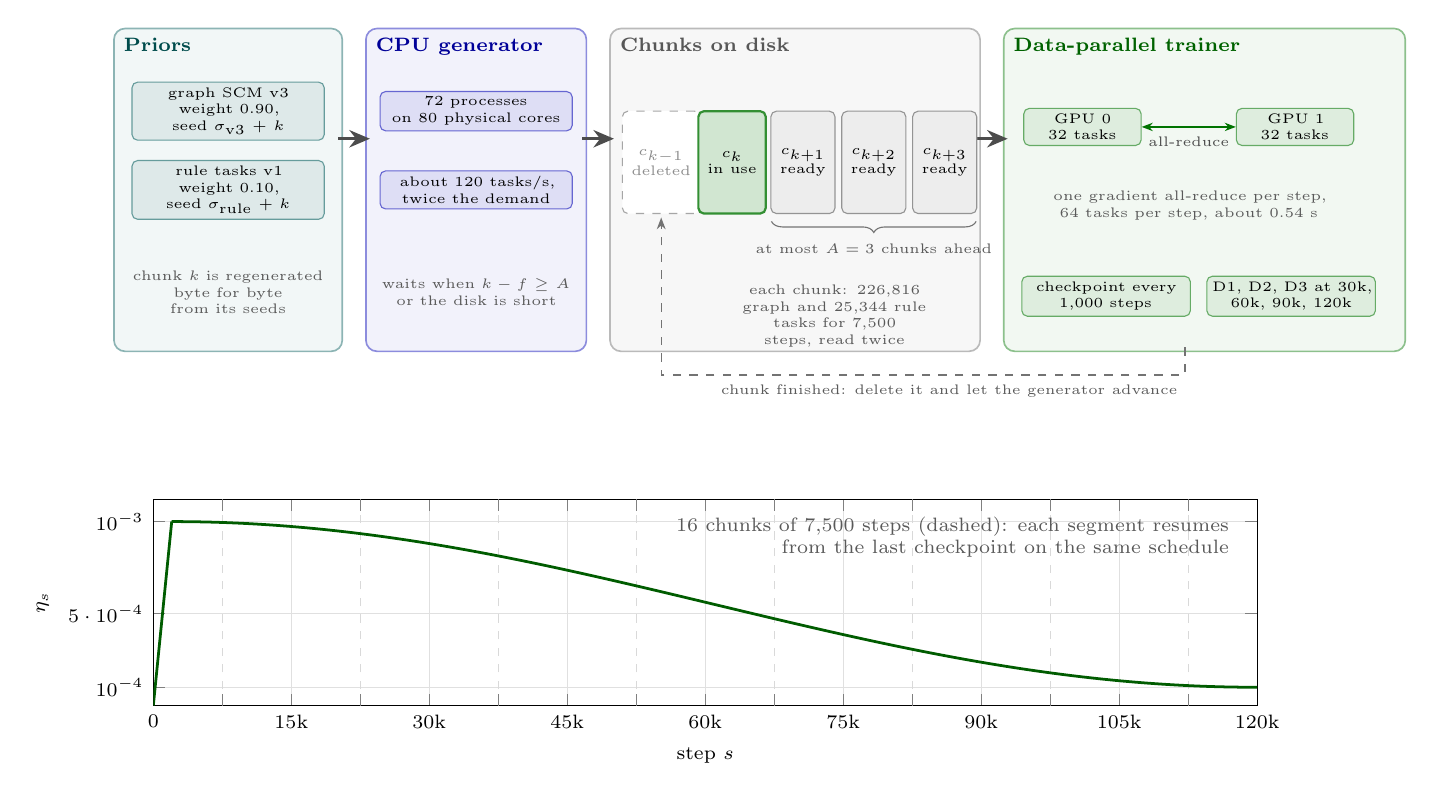
\begin{tikzpicture}[x=1cm, y=1cm]

% panels
\draw[panel=cdata] (0,2.9)    rectangle (2.9,7.0);
\draw[panel=ccell] (3.2,2.9)  rectangle (6.0,7.0);
\draw[panel=cin]   (6.3,2.9)  rectangle (11.0,7.0);
\draw[panel=cgpu]  (11.3,2.9) rectangle (16.4,7.0);
\foreach \a/\b in {2.9/3.2, 6.0/6.3, 11.0/11.3} \draw[bigflow] (\a-0.05,5.6) -- (\b+0.05,5.6);

% priors
\node[ptitle=cdata] at (0.12,6.88) {Priors};
\node[sbox=cdata, text width=2.3cm] at (1.45,5.95) {graph SCM v3\\weight 0.90, seed $\sigma_{\mathrm{v3}}+k$};
\node[sbox=cdata, text width=2.3cm] at (1.45,4.95) {rule tasks v1\\weight 0.10, seed $\sigma_{\mathrm{rule}}+k$};
\node[note, text width=2.5cm] at (1.45,3.65) {chunk $k$ is regenerated\\byte for byte from its seeds};

% generator
\node[ptitle=ccell] at (3.32,6.88) {CPU generator};
\node[sbox=ccell, text width=2.3cm] at (4.6,5.95) {72 processes\\on 80 physical cores};
\node[sbox=ccell, text width=2.3cm] at (4.6,4.95) {about 120 tasks/s,\\twice the demand};
\node[note, text width=2.5cm] at (4.6,3.65) {waits when $k-f\ge A$\\or the disk is short};

% chunks on disk
\node[ptitle=cin] at (6.42,6.88) {Chunks on disk};
\node[draw=black!35, dashed, fill=white, rounded corners=2pt, minimum width=0.78cm, minimum height=1.3cm,
      font=\tiny, text=black!45, align=center] at (6.95,5.3) {$c_{k-1}$\\deleted};
\node[draw=cgpu!80, fill=cgpu!18, rounded corners=2pt, minimum width=0.78cm, minimum height=1.3cm,
      font=\tiny, align=center, line width=0.8pt] at (7.85,5.3) {$c_{k}$\\in use};
\foreach \i/\l in {0/{k+1}, 1/{k+2}, 2/{k+3}}
  \node[draw=cin!70, fill=black!7, rounded corners=2pt, minimum width=0.78cm, minimum height=1.3cm,
        font=\tiny, align=center] at (8.75+\i*0.9,5.3) {$c_{\l}$\\ready};
\draw[decorate, decoration={brace, amplitude=4pt, mirror}, black!55] (8.35,4.55) -- (10.95,4.55);
\node[note] at (9.65,4.2) {at most $A=3$ chunks ahead};
\node[note, text width=3.3cm] at (9.15,3.35) {each chunk: 226,816 graph and 25,344 rule\\tasks for 7,500 steps, read twice};

% trainer
\node[ptitle=cgpu] at (11.42,6.88) {Data-parallel trainer};
\node[sbox=cgpu, text width=1.35cm] (g0) at (12.3,5.75) {GPU 0\\32 tasks};
\node[sbox=cgpu, text width=1.35cm] (g1) at (15.0,5.75) {GPU 1\\32 tasks};
\draw[{Stealth[length=1.4mm]}-{Stealth[length=1.4mm]}, line width=0.6pt, cgpu] (g0) -- node[below, font=\tiny, text=black!70] {all-reduce} (g1);
\node[note, text width=4.6cm] at (13.65,4.75) {one gradient all-reduce per step,\\64 tasks per step, about 0.54 s};
\node[sbox=cgpu, text width=2.0cm] at (12.6,3.6) {checkpoint every\\1,000 steps};
\node[sbox=cgpu, text width=2.0cm] at (14.95,3.6) {D1, D2, D3 at 30k,\\60k, 90k, 120k};

% feedback
\draw[flow, dashed, black!55] (13.6,2.95) -- (13.6,2.6) -- node[below, font=\tiny, text=black!65, pos=0.45] {chunk finished: delete it and let the generator advance} (6.95,2.6) -- (6.95,4.6);


% learning-rate schedule of the final run, computed from the formula in Section 5
\begin{axis}[at={(0.5cm,-1.6cm)}, anchor=south west, width=15.6cm, height=4.2cm,
  scaled y ticks=false,
  xmin=0, xmax=120000, ymin=0, ymax=1.12e-3,
  xtick={0,15000,30000,45000,60000,75000,90000,105000,120000},
  xticklabels={0,15k,30k,45k,60k,75k,90k,105k,120k},
  extra x ticks={7500,22500,37500,52500,67500,82500,97500,112500}, extra x tick labels={},
  extra x tick style={grid=major, major grid style={black!15, dashed}},
  ytick={1e-4,5e-4,1e-3}, yticklabels={$10^{-4}$,$5\cdot10^{-4}$,$10^{-3}$},
  xlabel={step $s$}, ylabel={$\eta_s$},
  grid=major, grid style={black!12},
  tick label style={font=\scriptsize}, label style={font=\scriptsize},
  scaled x ticks=false]
\addplot[cgpu!80!black, line width=1pt, domain=0:2000, samples=2] {1e-3*(x+1)/2000};
\addplot[cgpu!80!black, line width=1pt, domain=2000:120000, samples=240]
  {1e-3*(0.1+0.45*(1+cos(deg(pi*(x-2000)/118000))))};
\node[font=\scriptsize, text=black!65, anchor=north east, align=right] at (axis cs:118000,1.08e-3)
  {16 chunks of 7,500 steps (dashed): each segment resumes\\from the last checkpoint on the same schedule};
\end{axis}
\end{tikzpicture}
}
\caption{Training system of the final run. Top: CPU processes generate chunks of fresh tasks from
the priors, at most $A=3$ chunks ahead of the trainer; two GPUs train on the current chunk with one
gradient all-reduce per step, and every finished chunk is deleted. Bottom: the learning rate over
the 120,000 steps; the sixteen segments, one per chunk, resume from checkpoints and follow one
warmup and cosine schedule.}
\label{fig:pipeline}
\end{figure}

The final run uses $K=16$, $S_c=7{,}500$, $\tau=64$, $\mu_s=0.05$, $\Pi=2$ and the mixture of graph
v3 (90\%) and rule v1 (10\%), so each chunk holds $T_{\mathrm{v3}}=226{,}816$ and
$T_{\mathrm{rule}}=25{,}344$ tasks. Over 120,000 steps the model draws 7.68 million tasks from pools
containing 4.03 million distinct tasks. Generation runs on 72 CPU processes pinned to 80 physical cores and produces
about 120 tasks per second, roughly twice what the trainer consumes, with 16 cores reserved for training.

\section{Evaluation protocol}
\label{sec:eval}

Variants are compared on three sets that are disjoint from TabArena (Figure~\ref{fig:protocol}).

\begin{figure}[tbp]
\centering
% Selection protocol: three selection sets, paired statistics, TabArena kept for the final model.
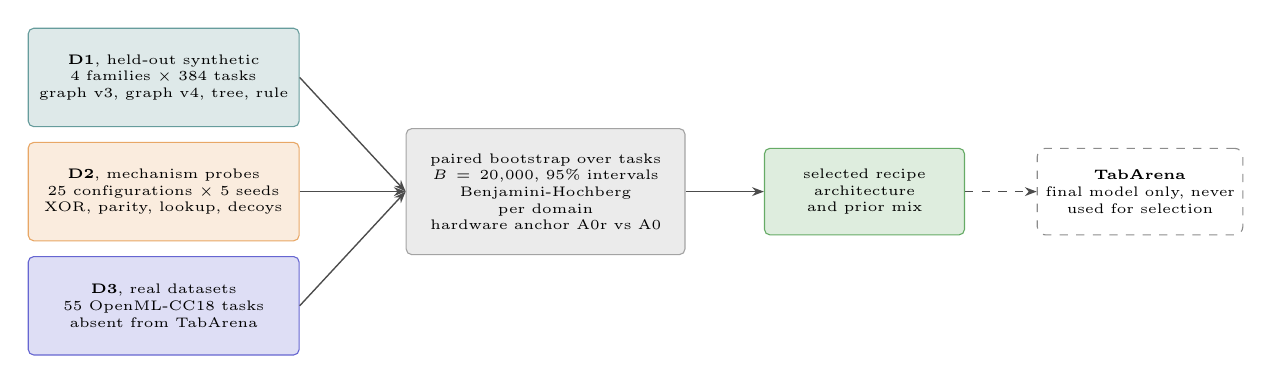
\begin{tikzpicture}[x=1cm, y=1cm]
\node[sbox=cdata, text width=3.3cm, minimum height=1.25cm] (d1) at (1.85,3.3)
  {\textbf{D1}, held-out synthetic\\4 families $\times$ 384 tasks\\graph v3, graph v4, tree, rule};
\node[sbox=cref, text width=3.3cm, minimum height=1.25cm] (d2) at (1.85,1.85)
  {\textbf{D2}, mechanism probes\\25 configurations $\times$ 5 seeds\\XOR, parity, lookup, decoys};
\node[sbox=ccell, text width=3.3cm, minimum height=1.25cm] (d3) at (1.85,0.4)
  {\textbf{D3}, real datasets\\55 OpenML-CC18 tasks\\absent from TabArena};
\node[sbox=cin, text width=3.4cm, minimum height=1.6cm] (st) at (6.7,1.85)
  {paired bootstrap over tasks\\$B=20{,}000$, 95\% intervals\\Benjamini-Hochberg per domain\\hardware anchor A0r vs A0};
\foreach \n in {d1,d2,d3} \draw[flow] (\n.east) -- (st.west);
\node[sbox=cgpu, text width=2.4cm, minimum height=1.1cm] (sel) at (10.75,1.85) {selected recipe\\architecture and prior mix};
\draw[flow] (st) -- (sel);
\node[draw=black!45, dashed, rounded corners=3pt, fill=white, font=\tiny, align=center,
      text width=2.4cm, minimum height=1.1cm, inner sep=3pt] (ta) at (14.25,1.85)
  {\textbf{TabArena}\\final model only, never used for selection};
\draw[flow, dashed] (sel) -- (ta);
\end{tikzpicture}

\caption{Selection protocol. Design decisions are taken on D1, D2 and D3 with paired statistics (the
long-context stage also on learning curves of the largest D3 datasets, Section~\ref{sec:large}); TabArena is
reserved for the final models.}
\label{fig:protocol}
\end{figure}

\begin{description}
\item[D1, held-out synthetic tasks.] Four families of 384 tasks each, graph v3, graph v4, tree and
rule, generated with a dedicated seed that differs from every training seed. Since the rule family
weighs 25\% of the D1 mean and only 10\% of the final training mixture, we read the families
separately and use the graph and tree families as guards.
\item[D2, mechanism probes.] Twenty-five probe configurations with five seeds each, 800 context rows
and 1,000 test rows, where the informative columns are placed among Gaussian distractors to reach
$d$ features. Probes include XOR of two features, parity of three, a depth-two tree rule, a sparse
linear control, lookup tables with 16 and 64 categories, heavy-tailed thresholds, ratios, and XOR
with near-duplicate decoy columns.
\item[D3, real datasets.] The 55 classification tasks of OpenML-CC18 \cite{bischl2021} with at most
ten classes that are absent from TabArena, by name or by matching row and class counts, excluding
image datasets. Each task is reduced to at most 1,000 rows and 100 random features and evaluated by
stratified five-fold cross-validation; AUC is averaged over folds, using one-vs-rest macro AUC for
multiclass tasks.
\end{description}

\paragraph{Paired statistics.} For two models $A$ and $B$ evaluated on the same $n$ tasks with scores
$a_t$ and $b_t$, we report $\Delta=\frac{1}{n}\sum_t(a_t-b_t)$ with a percentile interval from
$B=20{,}000$ bootstrap resamples of the tasks, and the two-sided p-value
\begin{equation}
p=\frac{1+\#\{b:\ |\Delta^{*}_b-\Delta|\ge|\Delta|\}}{B+1}.
\end{equation}
For D2, with five seeds per probe, the bootstrap enumerates all resamples and a sign-flip test gives
the p-value. Within every domain and metric, p-values are adjusted with the Benjamini-Hochberg
procedure \cite{benjamini1995}. All ablations use a single training seed, so the intervals capture
task sampling and leave out the variance across training runs; Section~\ref{sec:anchor} estimates the
latter through one hardware anchor rather than a repeated-seed variance estimate. An interval that includes
zero does not establish equivalence. Unless otherwise stated,
an AUC difference in points means 100 times the difference on the $[0,1]$ AUC scale. D1--D3 are selection
sets, so their results are not an independent final test of choices made with those sets.

\section{Experiments}
\label{sec:exp}

\subsection{Setup}
Ablations train for 8,000 steps of 32 tasks with warmup 800 and seed 0, which amounts to 256,000 task
draws. Series A and B ran on an AMD RX 7900 XT, series C on an RTX 5090. Unless stated otherwise, the
models are evaluated with one estimator. The runs are:
A0 (baseline architecture, graph v3 only); B1 (radial basis cell embedding);
B2 (auxiliary masked-cell reconstruction loss, weight 0.1); B3 (row summary mode);
B4 (B3 with row refinement and one ICL block less); A2 (A0 trained on graph v4 85\% and rule 15\%);
A3 (A2 with a stronger load-time augmentation); A0r (A0 repeated on the RTX 5090);
C1 and C2 (B3 and B4 trained on graph v3 90\% and rule 10\%); C3a and C3b (B4 and B3 trained on
graph v3 45\%, graph v4 45\% and rule 10\%).

\begin{table}[t]
\centering
\small
\begin{tabular}{llcccccc}
\toprule
& & \multicolumn{5}{c}{D1 (held-out synthetic)} & D3 \\
\cmidrule(lr){3-7}
Run & Change & graph v3 & graph v4 & tree & rule & mean & real \\
\midrule
A0  & baseline                          & .8755 & .8256 & .8308 & .7322 & .8160 & .8869 \\
A0r & A0 on another GPU                 & .8756 & .8250 & .8331 & .7281 & .8155 & .8900 \\
B1  & RBF cell embedding                & .8751 & .8262 & .8366 & .7337 & .8179 & .8897 \\
B2  & masked-cell auxiliary loss        & .8708 & .8242 & .8323 & .7220 & .8123 & .8870 \\
B3  & row summary                       & .8779 & .8269 & .8325 & .7317 & .8173 & .8897 \\
B4  & B3 + row refinement               & .8794 & .8351 & .8418 & .7302 & .8216 & .8921 \\
A2  & graph v4 85\% + rule 15\%         & .8643 & .8098 & .8180 & .7993 & .8228 & .8838 \\
A3  & A2 + augmentation                 & .8627 & .8177 & .8132 & .7691 & .8157 & .8819 \\
C1  & B3, v3 90\% + rule 10\%           & .8755 & .8251 & .8317 & .7751 & .8269 & .8859 \\
\rowcolor{orange!12}
C2  & B4, v3 90\% + rule 10\%           & .8791 & .8340 & .8408 & .8236 & .8444 & .8937 \\
C3a & B4, v3/v4 45\% + rule 10\%        & .8784 & .8301 & .8402 & .7721 & .8302 & .8901 \\
C3b & B3, v3/v4 45\% + rule 10\%        & .8731 & .8237 & .8296 & .7692 & .8239 & .8864 \\
\bottomrule
\end{tabular}
\caption{Mean AUC of all ablations after 8,000 steps, one estimator. C2 is the recipe of the final
run.}
\label{tab:abs}
\end{table}

\begin{table}[t]
\centering
\small
\begin{tabular}{lccc}
\toprule
Comparison & D1 mean & D1 rule & D3 \\
\midrule
A0r $-$ A0 & $-0.06\ [-0.22,\ 0.11]$ & $-0.41\ [-0.85,\ 0.01]$ & $+0.31\ [0.06,\ 0.54]$ \\
B4 $-$ A0 & $+0.56\ [0.34,\ 0.78]$ & $-0.20\ [-0.86,\ 0.48]$ & $+0.51\ [0.18,\ 0.84]$ \\
B4 $-$ B3 & $+0.44\ [0.23,\ 0.64]$ & $-0.15\ [-0.74,\ 0.47]$ & $+0.24\ [-0.18,\ 0.62]$ \\
A2 $-$ A0 & $+0.68\ [0.25,\ 1.13]$ & $+6.71\ [5.43,\ 8.03]$ & $-0.32\ [-0.82,\ 0.18]$ \\
C1 $-$ B3 & $+0.96\ [0.66,\ 1.27]$ & $+4.35\ [3.35,\ 5.38]$ & $-0.38\ [-0.78,\ -0.05]$ \\
C2 $-$ B4 & $+2.27\ [1.82,\ 2.74]$ & $+9.34\ [7.78,\ 10.94]$ & $+0.17\ [-0.15,\ 0.44]$ \\
C2 $-$ C1 & $+1.75\ [1.42,\ 2.10]$ & $+4.84\ [3.73,\ 6.02]$ & $+0.78\ [0.39,\ 1.18]$ \\
C3a $-$ C2 & $-1.41\ [-1.78,\ -1.08]$ & $-5.14\ [-6.40,\ -3.95]$ & $-0.37\ [-0.61,\ -0.15]$ \\
C3b $-$ C1 & $-0.30\ [-0.50,\ -0.11]$ & $-0.60\ [-1.18,\ -0.05]$ & $+0.05\ [-0.30,\ 0.42]$ \\
\bottomrule
\end{tabular}
\caption{Paired differences in AUC points with 95\% bootstrap intervals over tasks (1,536 D1 tasks,
384 rule tasks, 55 D3 tasks).}
\label{tab:paired}
\end{table}

\subsection{How large is a single-seed difference?}
\label{sec:anchor}
A0r repeats the recipe of A0 on a different GPU and software stack, which changes the floating-point
order of operations and therefore the training trajectory. On D1 the two runs agree within
0.06 points. On D3, A0r scores 0.31 points higher with an interval that excludes zero
(Table~\ref{tab:paired}). The external suite has only 55 tasks, and a change of trajectory alone moves
its mean by about 0.3 points in this comparison. We therefore interpret single-seed D3 differences of that
size cautiously and give more weight to D1, whose 1,536 tasks yield narrower task-bootstrap intervals.

\subsection{Architecture}
Among the architecture variants, only B4 produces a clear gain (Table~\ref{tab:paired}). It improves
the D1 mean by 0.56 points over A0, with the largest effects on graph v4 (+0.95) and tree tasks
(+1.10), and improves D3 by 0.51 points, mostly on multiclass tasks (+0.71). The gain over B3 on D1
(+0.44) concentrates on the same two families, while the D3 gain over B3 stays within the noise
level established above. The radial basis embedding of B1 helps only the tree family. The auxiliary
masked-cell loss of B2 gives no detectable D3 gain (0.8870 against 0.8869) and lowers the D1 mean;
at this training budget, we find no benefit for classification. The summary row mode of
B3 gives no clear accuracy difference from the baseline while cutting the training time per step by 30\%.
The B4 comparison changes three components together: row refinement, a second column stage and
ICL depth (eight to seven). The experiments identify the effect of this configuration, rather than
the isolated contribution of each added module.

\subsection{Priors and the interaction between prior and architecture}
Adding rule tasks teaches interactions, and how much the model learns depends on the row stage. With
graph v4 and 15\% rule tasks, A2 gains 6.7 points on the rule family and loses between 1.1 and 1.6
points on every other D1 family. Restricting the change to 10\% rule tasks on graph v3 removes most of
that cost: C2 improves on B4 by 9.3 points on rule tasks while the graph and tree families move by at
most 0.11 points in either direction, all within their intervals. The same mixture on the summary
architecture (C1) gains 4.4 points on rule tasks over B3, half of what B4 gains, and C2 beats C1 by
1.75 points on D1 and by 0.78 points on D3.

Figure~\ref{fig:probes} shows the same effect on the probes. With rule tasks, C2 solves XOR among 10
and 30 features, three-way parity among 10 features and XOR with near-duplicate decoys among 30
features (0.998, against 0.559 for A0), all with AUC of 0.97 or more. C1 and A2, which see rule tasks
with different architectures or mixtures, stay far below. The controlled C2--C1 comparison supports
an interaction between rule data and the B4 configuration: richer cell processing before compression
is a plausible explanation, but the row and column refinement contributions are not isolated.
The probes also mark the limit of this skill: C2 still reaches 0.82 on XOR among 50 features,
while parity among 30 features and XOR among 100 stay at chance for every model (0.51 and 0.54 for
C2).

Replacing half of the graph v3 tasks with graph v4 hurts (C3a against C2): the D1 mean drops by 1.41
points, mostly on rule tasks, D3 drops by 0.37 points with an interval below zero, and the probe gains
disappear. Graph v4 tasks are harder and more balanced, and the checkpoint trend of A2 suggests that
they are learned more slowly; at our budget they compete with skills that the other components
already provide. The final mixture therefore contains no graph v4 tasks.

\begin{figure}[tbp]
\centering
% D2 probes: AUC against the total number of features d (mean of five seeds, bars from the lowest
% to the highest seed). Data: plotdata/probe_*.dat from make_data.py.
\begin{tikzpicture}
\begin{groupplot}[
  group style={group size=2 by 1, horizontal sep=1.3cm},
  width=7.1cm, height=5.2cm,
  xmode=log, log basis x=10, minor xtick={},
  ymin=0.44, ymax=1.03, ytick={0.5,0.6,0.7,0.8,0.9,1.0},
  xlabel={features $d$ (informative and noise)},
  grid=major, grid style={black!12},
  tick label style={font=\scriptsize}, label style={font=\scriptsize}, title style={font=\small},
  every axis plot/.append style={line width=0.8pt, mark size=1.6pt},
  error bars/error bar style={line width=0.5pt},
  error bars/error mark options={rotate=90, mark size=1.5pt, line width=0.5pt},
  cycle list={
    {black!45, mark=o},
    {ccell, mark=square},
    {cref, mark=triangle},
    {ccol, mark=diamond},
    {crow, mark=*, line width=1.3pt},
    {cdec, mark=pentagon*, line width=1.3pt},
    {cdata, mark=star, line width=1.3pt, mark size=2.2pt}},
]
\nextgroupplot[title={XOR of two features}, ylabel={AUC},
  xtick={2,10,30,50,100}, xticklabels={2,10,30,50,100},
  legend style={font=\scriptsize, draw=black!30, legend columns=4, column sep=6pt,
                at={(1.09,-0.36)}, anchor=north}]
\draw[black!50, dashed, line width=0.5pt] (axis cs:1.8,0.5) -- (axis cs:115,0.5);
\pgfplotsinvokeforeach{A0,B4,A2,C1,C2,F30,F120}{
  \addplot+[error bars/.cd, y dir=both, y explicit] table[x=d, y=#1, y error plus=#1_hi, y error minus=#1_lo] {plotdata/probe_xor2.dat};}
\legend{A0, B4, A2, C1, C2 (final recipe), F30 (final run{,} 30k steps), F120 (120k steps)}
\nextgroupplot[title={parity of three features},
  xtick={3,10,30,100}, xticklabels={3,10,30,100}]
\draw[black!50, dashed, line width=0.5pt] (axis cs:2.7,0.5) -- (axis cs:115,0.5);
\pgfplotsinvokeforeach{A0,B4,A2,C1,C2,F30,F120}{
  \addplot+[error bars/.cd, y dir=both, y explicit] table[x=d, y=#1, y error plus=#1_hi, y error minus=#1_lo] {plotdata/probe_parity3.dat};}
\end{groupplot}
\end{tikzpicture}

\caption{D2 probes: AUC as the number of features $d$ grows, with two (XOR) or three (parity)
informative features and Gaussian noise in the others. Points are means over five seeds, bars span
the lowest and highest seed, the dashed line is chance. Among the ablations, only C2, which combines
the row refinement with rule tasks, solves XOR up to 30 features and parity up to 10. F30 and F120, the
final run after 30,000 and 120,000 steps (Section~\ref{sec:final}), extend XOR to 50 features; XOR among
100 features varies between checkpoints (0.81 for F30, 0.66 for F120) and parity among 30 features
stays close to chance.}
\label{fig:probes}
\end{figure}

\subsection{Training dynamics}
Figure~\ref{fig:trend} follows three runs across checkpoints. The lead of B4 over A0 is large early in
training, 8.3 points of D1 at 2,000 steps, and settles at about half a point by 8,000 steps. A2 trails
A0 at 4,000 steps (0.7731 against 0.8028) and then improves faster, with its rule AUC still rising by
2.6 points between 6,000 and 8,000 steps. Both observations indicate that 8,000 steps rank only the clear effects and
that some components may need much longer training to show their value, which motivates the long
final run.

\begin{figure}[tbp]
\centering
% EMA checkpoints at 2k, 4k, 6k and 8k steps: D1 mean, D1 rule family and D3 mean AUC.
% Data: plotdata/trend.dat from make_data.py.
\begin{tikzpicture}
\begin{groupplot}[
  group style={group size=3 by 1, horizontal sep=1.25cm},
  width=5.4cm, height=4.6cm,
  xtick={2000,4000,6000,8000}, xticklabels={2k,4k,6k,8k}, xmin=1600, xmax=8400,
  xlabel={training step},
  grid=major, grid style={black!12},
  tick label style={font=\scriptsize}, label style={font=\scriptsize}, title style={font=\small},
  yticklabel style={/pgf/number format/.cd, fixed, precision=2},
  every axis plot/.append style={line width=0.8pt, mark size=1.6pt},
  legend style={font=\scriptsize, draw=black!30, at={(0.97,0.03)}, anchor=south east, row sep=-1pt},
  cycle list={{black!45, mark=o}, {ccell, mark=square}, {cref, mark=triangle}},
]
\nextgroupplot[title={D1, mean of four families}, ylabel={AUC}]
\pgfplotsinvokeforeach{A0,B4,A2}{\addplot table[x=step, y=#1_d1] {plotdata/trend.dat};}
\legend{A0, B4, A2}
\nextgroupplot[title={D1, rule family}]
\pgfplotsinvokeforeach{A0,B4,A2}{\addplot table[x=step, y=#1_rule] {plotdata/trend.dat};}
\nextgroupplot[title={D3, 55 real datasets}]
\pgfplotsinvokeforeach{A0,B4,A2}{\addplot table[x=step, y=#1_d3] {plotdata/trend.dat};}
\end{groupplot}
\end{tikzpicture}

\caption{AUC of the EMA checkpoints after 2,000 to 8,000 steps of the ablations. B4 leads early and
keeps about half a point at the end; A2 (graph v4 and rule tasks) starts slower and is still rising
on the rule family when the ablation stops.}
\label{fig:trend}
\end{figure}

\subsection{Comparison with gradient-boosted trees}
\label{sec:gbdt}
Table~\ref{tab:gbdt} places LightPFN among default tree ensembles on D3, with the same paired bootstrap
as the ablations. After 256,000 synthetic tasks and with a single estimator, C2 has a higher mean AUC
than default random forest \cite{breiman2001}, LightGBM \cite{ke2017} and XGBoost \cite{chen2016}, but
none of the corresponding bootstrap intervals excludes zero ($+0.04$, $+0.30$ and $+1.19$ points), and it
is 0.86 points behind default CatBoost \cite{prokhorenkova2018} ($[-1.70,\ -0.19]$), with the higher
AUC on 27\% of the tasks. The final run closes and then reverses that gap. Its checkpoint after
30,000 steps, F30 (Section~\ref{sec:final}), has no clear mean AUC advantage over CatBoost: 0.31 points higher, with an
interval of $[-0.13,\ 0.73]$ that includes zero. The final checkpoint after 120,000 steps, F120, is
0.81 points above CatBoost ($[0.39,\ 1.29]$) with the higher AUC on 76\% of the tasks, on binary
($+0.72$) as well as multiclass tasks ($+0.89$), both with intervals above zero. F120 leads default
random forest, LightGBM and XGBoost by 1.70, 1.96 and 2.85 points, with intervals above zero and the
higher AUC on 85 to 93\% of the tasks. The 2.85-point XGBoost difference includes a failed run: on all
five folds of the OpenML task \emph{sick} (task 3021), the categorical-input wrapper creates a
categorical column with no observed training categories, which XGBoost rejects. The harness assigns
uniform predictions to the failed folds; their AUC of 0.5 is a failure penalty, not a fitted model's
predictive performance. On the 54 successful tasks, the paired lead of F120 is 1.99 points
$[1.28,\ 2.84]$, with means 0.9088 for F120 and 0.8889 for XGBoost. We use this successful-task
comparison for the predictive claim and retain the penalized result for transparency in
Table~\ref{tab:gbdt}. All D3 tasks have at most 1,000 training rows; Section~\ref{sec:large} turns to
larger tables.
An earlier model of the series, r2
(baseline architecture, 15,000 steps on graph v3), had been evaluated on the TabArena lite protocol
before the selection protocol was introduced: with four estimators it reached a mean AUC of 0.8290
against 0.8294 for default CatBoost, ahead of default LightGBM (0.8104) and XGBoost (0.7966). We report
it as a reference point and have not used TabArena for any decision since; Section~\ref{sec:tabarena}
evaluates the final models.

\begin{table}[t]
\centering
\small
\begin{tabular}{lccc}
\toprule
Model (D3, 55 tasks) & mean AUC & F120 $-$ model & F120 higher \\
\midrule
\rowcolor{orange!12}
LightPFN F120, final run at 120,000 steps & .9104 & & \\
LightPFN F30, final run at 30,000 steps & .9054 & $+0.49\ [0.17,\ 0.89]$ & 84\% \\
CatBoost, default & .9023 & $+0.81\ [0.39,\ 1.29]$ & 76\% \\
LightPFN C2, 8,000 steps & .8937 & $+1.66\ [1.03,\ 2.46]$ & 95\% \\
Random forest, default & .8933 & $+1.70\ [1.02,\ 2.51]$ & 85\% \\
LightGBM, default & .8907 & $+1.96\ [1.11,\ 3.07]$ & 91\% \\
XGBoost, default (54 successful tasks) & .8889 & $+1.99\ [1.28,\ 2.84]$ & 93\% \\
LightPFN A0, 8,000 steps & .8869 & $+2.34\ [1.72,\ 3.05]$ & 98\% \\
XGBoost, including failure penalty & .8819 & $+2.85\ [1.44,\ 5.01]$ & 93\% \\
\bottomrule
\end{tabular}
\caption{External suite D3 against default tree ensembles: one estimator for LightPFN, same splits for
every model. Differences in AUC points with 95\% bootstrap intervals; the last column is the share
of tasks on which F120 has the higher AUC. All rows use 55 tasks except the successful-task XGBoost
comparison, which excludes \emph{sick} from both models and has F120 mean AUC 0.9088. The last row
shows the 55-task result when the wrapper failure receives uniform predictions.}
\label{tab:gbdt}
\end{table}

\subsection{Cost}
\label{sec:cost}
On an RTX 5090, a training step of 32 tasks takes a median of 0.35 s for A0, 0.24 s for B3 trained
as C1 and 0.52 s for B4 trained as C2. On the CPU (AMD EPYC 9654, 16 threads, one estimator, shapes
from 800 context rows and 22 features up to 10,000 rows and 30 features), the fit and predict time of
B3 is 0.60 to 0.76 times that of A0 and the time of B4 is 1.24 to 1.38 times. We chose B4 because
its accuracy gain over B3 (0.8 points of D3 and 1.75 points of D1 with the final mixture) outweighs
a CPU cost about twice as high. Section~\ref{sec:large} reports timings for large tables on a shared
server, Section~\ref{sec:inference} a faster implementation of inference with the same predictions up to
floating-point rounding, and
Section~\ref{sec:tabarena} the cost on TabArena against the tree ensembles.

\section{Final run}
\label{sec:final}

The final model uses the C2 recipe: B4, graph v3 at 90\% and rule v1 at 10\%, no augmentation beyond
feature permutation and missingness. It trains for 120,000 steps of 64 tasks on two RTX 5090 GPUs with
the data-parallel scheme and the chunked stream of Section~\ref{sec:training}, warmup 2,000 steps and a
cosine schedule over the full run. A 300-step, three-chunk pilot verified recovery after an interrupted
training process, chunk deletion and schedule continuity. The full run took about 18 hours at
0.52--0.56 s per step. Checkpoints at 30,000, 60,000, 90,000 and 120,000 steps (F30, F60, F90 and F120)
were evaluated on D1, D2 and D3. TabArena was used only after the long-context stage had been selected
(Section~\ref{sec:tabarena}).

\subsection{Checkpoints from 30,000 to 120,000 steps}
After 30,000 steps, 1.92 million task draws and a quarter of the run, with the learning rate still at
88\% of its peak, F30 improves on C2 in every family of D1 and on D3 (Table~\ref{tab:final}). This
comparison measures the progress of the run rather than a design choice: F30 has seen 7.5 times as
many tasks as C2, with a batch twice as large and fresh data. The largest gain is on rule tasks, 6.65
points, followed by graph v3 (1.40), graph v4 (1.24) and tree tasks (1.10); on D3 the gain is 1.17
points.

The later checkpoints keep improving, with shrinking returns. The D1 mean rises from 0.8703 to 0.8746,
0.8773 and 0.8781, and D3 from 0.9054 to 0.9086, 0.9101 and 0.9104: on D3 each further quarter of the
run adds 0.32, 0.15 and 0.03 points. Between F60 and F120 every D1 family still gains, by 0.26 to 0.56
points with intervals above zero, and D3 gains 0.18 points $[0.05,\ 0.32]$. Over the whole run F120
improves on C2 by 3.38 points on D1 and 1.66 points on D3, with the higher AUC on 95\% of the external
tasks. The training loss, averaged over the last 500 steps before each checkpoint, goes from 0.398 to
0.386, 0.372 and 0.367. These diminishing gains do not establish convergence beyond this training budget;
the training tables have at most 2,048 rows.

The probes move the limit of the interaction skill outward (Figure~\ref{fig:probes}). XOR among 50
features rises from 0.815 for C2 to 0.994 at F30 and 1.000 at F120, three-way parity among 10 features
from 0.970 to 0.997, and the lookup table with 64 categories among 100 features from 0.858 to 0.896.
Parity among 30 features stays close to chance (0.50 to 0.54 across the checkpoints) and among 100 at
chance. XOR among 100 features is unstable: 0.807, 0.914, 0.825 and 0.656 at the four checkpoints, with
a wide spread over the five seeds, at the edge of what the model has learned.

\begin{table}[t]
\centering
\small
\begin{tabular}{lcccccc}
\toprule
& \multicolumn{5}{c}{D1 (held-out synthetic)} & D3 \\
\cmidrule(lr){2-6}
& graph v3 & graph v4 & tree & rule & mean & real \\
\midrule
C2, 8,000 steps $\times$ 32 tasks & .8791 & .8340 & .8408 & .8236 & .8444 & .8937 \\
F30, 30,000 steps $\times$ 64 tasks & .8930 & .8464 & .8518 & .8900 & .8703 & .9054 \\
F60, 60,000 steps & .8968 & .8526 & .8522 & .8969 & .8746 & .9086 \\
F90, 90,000 steps & .8991 & .8545 & .8540 & .9014 & .8773 & .9101 \\
\rowcolor{orange!12}
F120, 120,000 steps & .8994 & .8558 & .8549 & .9025 & .8781 & .9104 \\
\midrule
F120 $-$ C2 & $+2.03$ & $+2.18$ & $+1.41$ & $+7.89$ & $+3.38$ & $+1.66$ \\
{\footnotesize 95\% interval} & {\footnotesize $[1.59,\ 2.50]$} & {\footnotesize $[1.75,\ 2.65]$}
  & {\footnotesize $[1.09,\ 1.74]$} & {\footnotesize $[6.41,\ 9.40]$} & {\footnotesize $[2.95,\ 3.82]$}
  & {\footnotesize $[1.03,\ 2.46]$} \\
F120 $-$ F60 & $+0.26$ & $+0.32$ & $+0.27$ & $+0.56$ & $+0.35$ & $+0.18$ \\
{\footnotesize 95\% interval} & {\footnotesize $[0.09,\ 0.45]$} & {\footnotesize $[0.13,\ 0.52]$}
  & {\footnotesize $[0.05,\ 0.52]$} & {\footnotesize $[0.24,\ 0.95]$} & {\footnotesize $[0.23,\ 0.49]$}
  & {\footnotesize $[0.05,\ 0.32]$} \\
\bottomrule
\end{tabular}
\caption{Checkpoints of the final run (EMA weights, one estimator) against C2, the 8,000-step ablation
with the same recipe. Mean AUC and paired differences in AUC points with 95\% bootstrap intervals over
tasks.}
\label{tab:final}
\end{table}

\section{Large tables}
\label{sec:large}

\subsection{Learning curves on real datasets}
D3 reduces each dataset to at most 1,000 total rows before cross-validation, and pretraining tables have
at most 2,048 rows, so neither
shows how the model uses a long context. The scale test takes the 15 D3 datasets with at least 5,000
rows. For each dataset and each of two repeats it draws a stratified test set of $\min(2000,n/5)$ rows
and, from the remaining rows, stratified training sets of 1,000, 2,000, 4,000, 8,000, 16,000 and
32,000 rows where the dataset is large enough (15, 15, 15, 9, 6 and 6 datasets), plus one with all
remaining rows (4,324 to 94,320, median 8,992); at most 100 random features are kept, as in D3.
LightPFN reads the whole training set as context (full context) or, as in pretraining, stratified
subsamples of 2,048 rows, averaged over eight estimators. The tree ensembles use default settings.
Differences are averaged over the repeats of each dataset and bootstrapped over datasets.

With full context, the mean AUC difference between F120 and default CatBoost is inconclusive at
1,000 and 2,000 training rows and F120 falls
behind as the training set grows (Figure~\ref{fig:scale}, Table~\ref{tab:scale}): by 0.36 points at
4,000 rows, 0.64 at 8,000, 1.48 at 16,000 and 1.92 at 32,000, with intervals below zero from 8,000
rows, and by 0.77 points with all rows. The deficit has halved since F30 ($-3.52$ points at 32,000
rows), so longer pretraining on short tables also improves the use of long contexts, but it does not
remove the gap. The mean differences of LightGBM and XGBoost from CatBoost have intervals that include
zero at every size. From 4,000 rows up, the
full context beats eight subsamples of 2,048 rows, so the model extracts information from rows beyond
its pretraining length, but it gains less from them than the trees do. Where the training set fits in
2,048 rows, the eight estimators differ only in their feature orders and label slots and add 0.16 to
0.22 points. On 24 threads of a shared AMD EPYC server, fit and predict with full context take a median of
3.8 s at 16,000 rows and 11.6 s at 32,000, against 7.7 and 14.0 s for CatBoost; the in-context
attention grows quadratically with the context.

\begin{figure}[tbp]
\centering
% Scale test: AUC difference to default CatBoost against the number of training rows (mean over the large D3
% tasks, bars: 95% bootstrap interval over tasks). Data: plotdata/scale.dat from make_data.py.
\begin{tikzpicture}
\begin{axis}[
  width=11.5cm, height=6.4cm,
  xmode=log, log basis x=2, xmin=850, xmax=38000,
  xtick={1000,2000,4000,8000,16000,32000}, xticklabels={1k,2k,4k,8k,16k,32k}, minor xtick={},
  ymin=-6.4, ymax=1.3, ytick={-6,-5,-4,-3,-2,-1,0,1},
  xlabel={training rows}, ylabel={AUC $-$ default CatBoost (points)},
  grid=major, grid style={black!12},
  tick label style={font=\scriptsize}, label style={font=\scriptsize},
  every axis plot/.append style={line width=0.8pt, mark size=1.6pt},
  error bars/error bar style={line width=0.5pt},
  error bars/error mark options={rotate=90, mark size=1.5pt, line width=0.5pt},
  legend style={font=\scriptsize, draw=black!30, at={(0.5,-0.2)}, anchor=north, legend columns=2,
                column sep=6pt, row sep=-1pt},
]
\draw[black!50, dashed, line width=0.5pt] (axis cs:850,0) -- (axis cs:38000,0);
\addplot[black!35, mark=o, densely dotted] table[x=size, y=LightGBM] {plotdata/scale_sizes.dat};
\addplot[black!35, mark=x, densely dotted] table[x=size, y=XGBoost] {plotdata/scale_sizes.dat};
\addplot[cref, mark=triangle, dashed] table[x=size, y=F30] {plotdata/scale_sizes.dat};
\addplot[ccell, mark=diamond, dashed] table[x=size, y=F120x8] {plotdata/scale_sizes.dat};
\addplot[crow, mark=*, line width=1.2pt, error bars/.cd, y dir=both, y explicit]
  table[x=size, y=F120, y error plus=F120_hi, y error minus=F120_lo] {plotdata/scale_sizes.dat};
\addplot[cdec, mark=pentagon, dashed] table[x=size, y=LC7k] {plotdata/scale_sizes.dat};
\addplot[cdata, mark=star, mark size=2.2pt, line width=1.2pt, error bars/.cd, y dir=both, y explicit]
  table[x=size, y=LC11k, y error plus=LC11k_hi, y error minus=LC11k_lo] {plotdata/scale_sizes.dat};
\legend{LightGBM, XGBoost, F30 (full context), F120 (8 subsamples of 2{,}048), F120 (full context),
        long-context stage{,} 11k steps, long-context stage{,} final (39k steps)}
\end{axis}
\end{tikzpicture}

\caption{Scale test on the 15 D3 datasets with at least 5,000 rows: AUC difference to default CatBoost
against the number of training rows (15 datasets up to 4,000 rows, 9 at 8,000, 6 at 16,000 and
32,000). Bars: 95\% bootstrap intervals over datasets. The long-context stage removes most of the gap
of the pretrained model F120: after 11,000 steps (tables of up to 10,240 rows, then up to 60,000) and at
its end after 39,250 steps. The curve of the final checkpoint is close to the one at 11,000 steps.}
\label{fig:scale}
\end{figure}

\begin{table}[t]
\centering
\footnotesize
\setlength{\tabcolsep}{4pt}
\begin{tabular}{lcccccccccc}
\toprule
& & CatBoost & \multicolumn{8}{c}{AUC $-$ default CatBoost (points)} \\
\cmidrule(lr){4-11}
rows & sets & AUC & F30 & F120 & 95\% interval & F120$\times$8 & LC11k & LC39k & 95\% interval & LGBM / XGB \\
\midrule
1,000 & 15 & .8959 & $-0.38$ & $+0.26$ & $[-0.13,\ 0.72]$ & $+0.42$ & $+0.42$ & $+0.46$ & $[0.13,\ 0.95]$ & $-0.01$ / $-0.20$ \\
2,000 & 15 & .9071 & $-0.71$ & $+0.10$ & $[-0.27,\ 0.46]$ & $+0.32$ & $+0.37$ & $+0.51$ & $[0.22,\ 0.84]$ & $+0.05$ / $-0.14$ \\
4,000 & 15 & .9187 & $-1.14$ & $-0.36$ & $[-0.78,\ 0.03]$ & $-0.40$ & $+0.20$ & $+0.33$ & $[-0.08,\ 0.74]$ & $+0.20$ / $+0.04$ \\
8,000 & 9 & .9085 & $-1.62$ & $-0.64$ & $[-1.33,\ -0.14]$ & $-0.95$ & $+0.05$ & $+0.15$ & $[-0.42,\ 0.74]$ & $+0.25$ / $+0.19$ \\
16,000 & 6 & .8723 & $-3.11$ & $-1.48$ & $[-2.82,\ -0.58]$ & $-2.14$ & $-0.38$ & $-0.38$ & $[-1.70,\ 0.92]$ & $+0.10$ / $-0.12$ \\
32,000 & 6 & .8784 & $-3.52$ & $-1.92$ & $[-3.41,\ -0.86]$ & $-2.72$ & $-0.43$ & $-0.42$ & $[-1.41,\ 0.70]$ & $+0.18$ / $+0.36$ \\
all & 15 & .9313 & $-1.81$ & $-0.77$ & $[-1.63,\ -0.09]$ & $-1.34$ & $+0.23$ & $+0.31$ & $[-0.23,\ 0.86]$ & $-0.01$ / $+0.10$ \\
\bottomrule
\end{tabular}
\caption{Scale test against default CatBoost. F30 and F120: checkpoints of the final run with full
context, and F120$\times$8 averaged over eight subsamples of 2,048 rows; LC11k and LC39k: the long-context
stage after 11,000 steps and at its end (39,250 steps), full context; LGBM and XGB: default LightGBM and XGBoost. Each
dataset is the mean of two repeats; intervals bootstrap the datasets.}
\label{tab:scale}
\end{table}

\subsection{Long-context stage}
As in the second stage of TabICLv2 \cite{tabiclv2}, training continues on longer tables from the final
checkpoint, with its weights, moving average and optimizer state, a new warmup of 200 steps and a
learning rate of $10^{-4}$ decaying with a cosine to $10^{-5}$. The mixture holds about a third of the
tasks from each of three pool families, all with graph v3 at 90\% and rule v1 at 10\%: the pretraining
pools (256 to 2,048 rows), kept so that the stage does not forget the regime in which F120 beats
CatBoost; medium tables of 1,024 to 10,240 rows in groups of four; and long tables of 4,096 to 60,000
rows in groups of two. For the medium and long tables the number of features is drawn log-uniformly
between 2 and 100, independently of the rows, since the pretraining geometry would give almost every
long table 100 features; the long tables also cap rows times features at 800,000, so they are narrow,
as long real tables often are. By groups, the mixture weights are 15\%, 35\% and 50\%. The long tables
are generated while the stage trains, and training restarts every 2,500 steps to read the new ones, so
it sees mostly fresh tables.

Long tables require row attention to be split into chunks of at most 32,768 rows to avoid the CUDA
kernel's 65,535-block grid limit. They also require a micro-batch budget that includes row overhead.
A forward-and-backward memory probe gives
\begin{equation}
M(n,m)\approx 0.09+1.77\times10^{-5}\,n\,(m+7.65)\ \text{GB}
\end{equation}
for $n$ rows and $m$ features. Groups are therefore split by $n(m+8)$ with a budget of
$1.1\times10^6$ (about 20 GB), counting real rather than padded features. Tasks above the budget are
subsampled, preserving the context fraction and stratifying context labels.

A kernel failure triggered a fallback to pretraining and medium pools for the first 7,000 steps;
only the remaining steps use all three families. A loader audit over 800 groups recovered task shares
of 32, 40 and 28\%, with long tables reaching 59,762 rows (median 16,307); the row cap removed no rows
in that audit. The stage was extended twice to 39,250 steps. Extensions stretched the remaining cosine
schedule and raised the restart learning rate by up to $3.4\times10^{-5}$; medium tables were generated
further to keep reuse near two reads. These changes are part of the training recipe evaluated here.

\paragraph{Results.} After its first 7,000 steps, on tables of at most 10,240 rows, the
checkpoint LC7k improves on F120 at every size of the scale test: by 0.47 points at 4,000 rows
$[0.17,\ 0.82]$, 0.55 at 8,000, 0.91 at 16,000 and 1.27 at 32,000 $[0.55,\ 1.96]$, and by 0.78 points
with all rows (15 of 15 datasets). The largest gain is at 32,000 rows, three times the longest table seen
at that point. After 11,000 steps, the last 3,750 of them with long tables, LC11k gains more, and the
final checkpoint (LC39k, 39,250 steps, the last of the run, not chosen among checkpoints) has about the
same curve: against F120 it is better by 0.20 points at 1,000 rows, 0.41 at 2,000, 0.69 at 4,000, 0.79
at 8,000, 1.10 at 16,000, 1.50 at 32,000 $[0.47,\ 2.59]$ and 1.08 with all rows $[0.43,\ 1.79]$. Against
CatBoost it is above at 1,000 and 2,000 rows ($+0.46$ and $+0.51$, intervals above zero), with intervals
that include zero from 4,000 to 32,000 rows ($-0.42$ at 32,000) and 0.31 points above it with all rows
(Table~\ref{tab:scale}). The checkpoints from 11,000 to 39,250 steps differ by at most 0.4 points
at 16,000 and 32,000 rows, with six datasets; most of the gain came in the first 11,000 steps and the
remaining 28,000 steps, with the decay of the learning rate to $10^{-5}$, add little. On the short tables
no clear change is detected: LC39k differs from F120 on D1 (0.8783 against 0.8781, $+0.01$ points, $[-0.07,\ 0.10]$) and
on D3 (0.9109 against 0.9104, $+0.06$ points, $[-0.08,\ 0.21]$), where it is 0.86 points above default
CatBoost $[0.42,\ 1.40]$, 2.02 above LightGBM and 1.76 above random forest, all with intervals above zero.
Against XGBoost on the 54 successful tasks, it leads by 2.06 points $[1.32,\ 2.94]$; the 55-task comparison
including the wrapper failure penalty gives 2.91 points and is not used as the predictive claim.
XOR among 100 features rises from 0.66 to 0.81 (0.88 at 11,000 steps; five seeds,
unstable at the edge of the trained width), XOR among up to 50 features and parity among 10 stay solved,
and parity among 30 stays at chance.

The all-rows condition includes six datasets with 32,000 to 94,000 training rows. LC39k beats the three
tree ensembles on \emph{electricity} (0.979 against 0.959 for CatBoost, 0.953 for LightGBM and 0.974 for
XGBoost), matches them on \emph{nomao}, trails CatBoost by 0.7 and 0.4 points on \emph{adult} and
\emph{jungle-chess}, and by 2.1 points on \emph{connect-4} with 66,000 rows, where it gained 3.5 points
over F120; \emph{numerai28.6} is close to chance for every model. Fit and predict take 75 s at 94,000
rows against 10 s for CatBoost, and 57 s against 365 s on the three-class \emph{connect-4}.

\paragraph{Large datasets outside the selection sets.} D4 (\texttt{lightpfn.eval.large}) takes 13 OpenML
datasets of 50,000 to 2.2 million rows from the AMLB and Grinsztajn suites that are neither in TabArena
nor in D3 (covertype, airlines, albert, jannis, volkert, shuttle, MiniBooNE, kick, okcupid-stem,
sf-police-incidents, porto-seguro, Higgs, road-safety). Each model is trained on 10,000, 25,000, 50,000
and 100,000 rows where the dataset is large enough (13, 13, 12 and 8 datasets) and tested on 5,000 rows,
one repeat, with the tree ensembles at default settings (Table~\ref{tab:large}). F120 is below
CatBoost at every size and significantly so from 50,000 rows ($-1.53$ points, $-2.20$ at 100,000).
The final long-context checkpoint is better than F120 on every dataset at every size: by 0.93 points
at 10,000 rows, 1.13 at 25,000, 1.33 at 50,000 and 1.86 at 100,000 rows $[1.02,\ 2.90]$, so the gain grows with
the training set, up to a size beyond the longest table seen in training (60,000 rows). Against CatBoost
the interval of the mean difference includes zero at every size, with higher AUC on 7 of 13, 5 of 13, 6 of 12 and 3 of 8
datasets. It leads on \emph{porto-seguro} ($+3.0$ to $+4.2$ points), \emph{jannis}, \emph{covertype} and \emph{Higgs}
and is level on \emph{MiniBooNE} and \emph{shuttle}; it trails on \emph{albert} ($-1.6$ to $-3.7$),
\emph{road-safety} ($-1.9$ to $-3.6$), \emph{kick} ($-1.0$ to $-2.0$) and, at 50,000 rows and more,
\emph{sf-police-incidents} and \emph{airlines}. Default LightGBM and XGBoost have a mean AUC 2.6 to 4.6 points
below it up to 50,000 rows; at 100,000 rows XGBoost is 2.2 points below it and LightGBM, 0.5 points below, is closer.
Fit and predict take a median of 4.4, 14, 40 and 106 s at 10,000 to 100,000 rows on 24 threads of the shared
server, against 21, 31, 40 and 74 s for CatBoost at the same settings.

\begin{table}[t]
\centering
\footnotesize
\setlength{\tabcolsep}{3pt}
\begin{tabular}{lccccccc}
\toprule
rows & sets & CatBoost AUC & LC39k AUC & F120 $-$ CatBoost & LC39k $-$ CatBoost & 95\% interval & LGBM / XGB $-$ CatBoost \\
\midrule
10,000 & 13 & .8141 & .8168 & $-0.65$ & $+0.28$ & $[-0.53,\ 1.20]$ & $-4.33$ / $-3.30$ \\
25,000 & 13 & .8225 & .8234 & $-1.03$ & $+0.09$ & $[-0.81,\ 1.08]$ & $-3.52$ / $-2.72$ \\
50,000 & 12 & .8311 & .8291 & $-1.53$ & $-0.20$ & $[-1.17,\ 0.76]$ & $-4.01$ / $-2.78$ \\
100,000 & 8 & .8027 & .7993 & $-2.20$ & $-0.34$ & $[-1.95,\ 1.29]$ & $-0.83$ / $-2.51$ \\
\bottomrule
\end{tabular}
\caption{D4, large datasets outside TabArena and D3: AUC difference to default CatBoost in points, mean
over datasets with a 95\% bootstrap interval; the AUC columns are means over datasets. F120: the pretrained model before the
long-context stage; LC39k: its final checkpoint; LGBM and XGB: default LightGBM and XGBoost.}
\label{tab:large}
\end{table}

The 15 datasets of the scale test also motivated the stage, but D4 did not enter its design, and the final
checkpoint is the last one of the run; TabArena remains the independent test.

\section{Inference}
\label{sec:inference}

Fitting encodes the context of each estimator once; prediction passes the query rows through the cell stages and
attends to the cached context (Section~\ref{sec:model}). Every result up to Section~\ref{sec:large}, and the
initial TabArena evaluations of Section~\ref{sec:tabarena}, use an implementation that runs each stage on the whole
table at once. Three changes lower the cost without changing the function that is computed. They are the defaults
of the classifier, and \texttt{chunk\_cells=None, batch\_cells=0, fold=False} restores the earlier path.

\paragraph{Cache-blocked cell stages.} The column stages treat every column independently, and row refinement
and row compression treat every row independently. A table of $n\times m$ cells can therefore be processed in
pieces: groups of whole columns for the column stages and groups of whole rows for the row stages, written into
one preallocated buffer, with the inducing-point caches of the column stages reassembled in their original order.
With pieces of about 1,024 cells per CPU thread, the activations of a piece stay in the processor caches instead
of streaming the whole table through memory at every operation. Each column and each row receives the same inputs
as before; only the blocking of the matrix products changes. The in-context stage, which needs all context rows
together, is unchanged. On the GPU the pieces hold about one million cells and only cap the memory.

\paragraph{Folded copy.} The classifier keeps a copy of the network in which the weight of every RMSNorm is
multiplied into the linear map that reads its output: the query, key-value and first feed-forward projections of
every block, and the query and key projections of the decoder after the last in-context norm. The normalization
left behind has no parameters. In the blocks with rotary embeddings, the query and key dimensions of every head
are permuted so that each rotation acts on adjacent pairs and becomes one complex multiplication. The copy
computes the same function with a different order of floating-point operations.

\paragraph{Estimators batched on the GPU.} On the GPU, the $E$ estimators of a fit are encoded and queried as one
batch of up to about four million cells. On the CPU they stay sequential: once the pieces fit in cache, batching
gave no further gain. The random draws of each estimator (context subsample, feature order, label slots) follow
the same sequence as before, which a test checks, and the probabilities are still summed estimator by estimator in
double precision.

\paragraph{Equivalence.} Tests compare each path with the plain one on randomly initialized networks, with
missing values and constant columns: cache blocking and the folded copy in five configurations (logits within
$2\cdot10^{-5}$), cache blocking with zero-padded features and with double-precision inputs, and the classifier
with seven combinations of the three changes in two configurations (probabilities within $10^{-6}$, same predicted
classes).
On the first fold of the 38 TabArena classification tasks at full size, cache blocking alone returns bitwise
identical probabilities on 36 tasks and differences below $6\cdot10^{-8}$ on the other two. On the GPU, batching
and folding together change the probabilities by at most $6.8\cdot10^{-6}$, with the same predicted class in every
row. Both TabArena protocols were rerun with the new defaults, on the CPU and on the GPU
(Section~\ref{sec:tabarena}): every rank is the same to the fourth decimal.

\paragraph{Speed and memory.} Table~\ref{tab:infer} times binary synthetic tables with four estimators on eight
threads pinned to eight cores of the EPYC 9654 server, one job at a time, best of two repeats. Fit plus predict
takes 1.1 to 4.1 times less time and peak memory falls by up to 2.3 times. Cache blocking gives most of the gain
and the folded copy adds 2 to 14\%. The gain grows with the number of cells per row and is largest with 200
features, where the plain cell stages are limited by memory traffic. With AVX2 kernels, the instruction set of
many laptop CPUs, the speedups are 1.07 to 4.0. On long tables with few features most of the prediction time is
the attention of the query rows over the cached context, which the changes leave as it is: with 20,000 context
rows, 10 features, 20,000 query rows and one estimator, prediction takes 5.9 to 6.0 s with both implementations
(best of three, two alternating runs of each), while fitting takes 5.3 to 5.4 s instead of 6.7 s and peak memory
falls from 1.4 to 1.05 GB. On an RTX 5090 the estimator batch makes the two smallest tables 1.9 and 3.2 times
faster and the others 7 to 27\% faster.

\begin{table}[t]
\centering
\footnotesize
\setlength{\tabcolsep}{4pt}
\begin{tabular}{lccccccc}
\toprule
& \multicolumn{4}{c}{CPU, 8 threads: fit $+$ predict (s)} & \multicolumn{2}{c}{peak memory (GB)} & GPU (ms) \\
\cmidrule(lr){2-5}\cmidrule(lr){6-7}\cmidrule(lr){8-8}
train $\times$ features $\times$ test & plain & fast & speedup & AVX2 & plain & fast & plain / fast \\
\midrule
500 $\times$ 10 $\times$ 250 & 0.34 & 0.31 & 1.10 & 1.07 & 0.75 & 0.76 & 64 / 20 \\
1,000 $\times$ 50 $\times$ 500 & 2.14 & 1.25 & 1.71 & 1.53 & 0.95 & 0.82 & 63 / 34 \\
3,000 $\times$ 30 $\times$ 1,500 & 5.12 & 2.92 & 1.75 & 1.74 & 1.10 & 0.85 & 105 / 83 \\
2,500 $\times$ 200 $\times$ 1,250 & 41.7 & 10.2 & 4.08 & 4.00 & 2.07 & 1.17 & 334 / 293 \\
10,000 $\times$ 20 $\times$ 5,000 & 24.1 & 13.9 & 1.73 & 1.65 & 1.40 & 1.01 & 446 / 372 \\
20,000 $\times$ 100 $\times$ 2,000 & 151.7 & 53.8 & 2.82 & 2.75 & 5.94 & 2.53 & 1,589 / 1,480 \\
\bottomrule
\end{tabular}
\caption{Inference cost on binary synthetic tables with four estimators. CPU: AMD EPYC 9654, eight threads on
eight cores, one job at a time, best of two repeats, AVX-512 kernels; plain is the implementation used for every
earlier result, fast the new defaults (cache blocking and folded copy); AVX2 is the same speedup with AVX2
kernels on the same machine; memory is the peak resident memory of the process. GPU: one RTX 5090, plain against
fast (estimator batch and folded copy).}
\label{tab:infer}
\end{table}

\subsection{Vulkan backend}
\label{sec:vulkan}
PyTorch reaches NVIDIA GPUs through CUDA and AMD GPUs through ROCm, which covers Linux and a subset of consumer
cards; Intel GPUs and most integrated GPUs are left out. The package therefore has a second GPU backend built on
Vulkan, which current GPU drivers support on Linux and Windows. It computes the folded network of the previous
section, with the same two calls (encode a context, predict query rows), through eight compute kernels written in
WGSL and compiled to SPIR-V by wgpu when the backend starts, so no SDK or compiler is needed on the user's machine:
a tiled matrix product with optional fused normalization, bias, GELU and residual; tiled attention with an online
softmax for long key sequences; an attention kernel for the few summary and inducing tokens; row normalization;
the cell features; rotary embeddings; the learned query scaling; and a strided copy. Kernels address tensors
through strided views, so the same kernel reads a column of cells, a row of cells or the leading tokens of every
row without copies. The column statistics and rank lookups (a sort and a binary search per column) stay on the
host in PyTorch, and the context stays in GPU memory between fit and prediction. Everything runs in float32;
sine, cosine and erf use their own range reduction and polynomial approximations (error below $5\cdot10^{-7}$),
so results do not depend on the precision of a driver's transcendental functions. Drivers reset a GPU whose job
runs too long (2 s on Windows; during development a 20,000-row encode submitted as one job triggered a ring reset
of the Linux amdgpu driver), so heavy dispatches are cut into slices of workgroups submitted in jobs of about
$5\cdot10^{10}$ floating-point operations.

Tests compare the backend with the PyTorch path on random networks with missing values, constant columns, padded
features and several architecture variants: logits agree within about $10^{-6}$ and classifier probabilities within
$3\cdot10^{-5}$. Table~\ref{tab:vulkan} times fit plus predict on an AMD RX 7900 XT: the backend is 6.0 to 10.3
times faster than the 16 threads of the host CPU and as fast as PyTorch with ROCm on the same GPU, or faster. One
estimator's training cells must fit a single GPU buffer (2 GB, about 8.4 million cells); above that the classifier
falls back to the CPU. Two general compilers were tried first: IREE had no attention lowering for Vulkan and
generated incorrect code for RDNA3 on part of the network, and ONNX Runtime's WebGPU provider computed the fused
attention with errors of 2 to 17\%.

\begin{table}[t]
\centering
\footnotesize
\begin{tabular}{lcccc}
\toprule
train rows $\times$ features, test rows & CPU, 16 threads & ROCm & Vulkan & Vulkan vs CPU \\
\midrule
1,000 $\times$ 20, 500 & 0.45 s & 0.057 s & 0.044 s & 10.3$\times$ \\
5,000 $\times$ 50, 2,000 & 4.84 s & 0.59 s & 0.50 s & 9.6$\times$ \\
10,000 $\times$ 100, 5,000 & 19.8 s & 2.48 s & 2.13 s & 9.3$\times$ \\
20,000 $\times$ 50, 5,000 & 29.2 s & 4.76 s & 4.86 s & 6.0$\times$ \\
20,000 $\times$ 200, 10,000 & 70.4 s & 10.4 s & 8.68 s & 8.1$\times$ \\
\bottomrule
\end{tabular}
\caption{Fit plus predict time of the B4 architecture with four estimators on synthetic binary tables: Intel
i7-13700KF (16 threads), and an AMD RX 7900 XT through PyTorch 2.13 with ROCm 7.2 or through the Vulkan backend
(Mesa RADV driver, Linux).}
\label{tab:vulkan}
\end{table}

\subsection{Software package}
The package (\texttt{pip install lightpfn}) exposes the model as a scikit-learn classifier: \texttt{fit} validates
the data and encodes the context, \texttt{predict\_proba} runs the query rows, and the estimator works with
pipelines, cloning and grid search. It accepts pandas data frames: columns of categorical, string, object or
Boolean type become ordinal codes of the categories seen in training, with missing values and unseen categories
as missing values. \texttt{device="auto"} picks a CUDA or ROCm GPU through PyTorch, then a Vulkan GPU, then the
CPU. The weights are downloaded as safetensors with a JSON configuration from a Hugging Face commit pinned in the
package; local checkpoints are read with PyTorch's restricted weights-only loader, and no code from a model
repository is ever executed. The wheel holds only the inference code and depends on PyTorch, NumPy, scikit-learn,
huggingface-hub and safetensors; the source repository also holds the priors, the trainer and the evaluation
harness of this report.

\section{TabArena}
\label{sec:tabarena}

TabArena \cite{tabarena} is the benchmark that the selection protocol keeps aside. Version 0.1 has 51 tasks; we
use its 38 classification tasks (30 binary, 8 multiclass). LightPFN has no regression head and none of the 13
regression tasks was evaluated. Only the two finalists of the final run are tested, F120 and its long-context
continuation LC39k, after the choice between them had been made on D1, D3 and the scale test. This is the first
look at TabArena for this series, and no decision in this report depends on it.

\subsection{Evaluation with our harness}

\paragraph{Protocol.} Our harness (\texttt{lightpfn.eval.harness}) runs two protocols. The lite protocol reduces
every task to at most 1,000 rows, stratified, and 100 random features, and evaluates it by stratified five-fold
cross-validation (190 splits). The full protocol uses the official OpenML splits on the complete tables, from 748
to 150,000 rows and up to 1,776 features, with the first repeat only (three folds, 114 splits), where TabArena
averages three or ten repeats. Above 20,000 training rows, which happens on 8 tasks, LightPFN subsamples its
context with stratification. The baselines are CatBoost, LightGBM, XGBoost and random forest at default settings,
run by the same harness, and TabICLv2 \cite{tabiclv2} (28M parameters, tabicl 2.2.0, default settings, on a GPU).
These evaluations do not reproduce the official leaderboard protocol, which includes default, tuned and
ensembled entries and ranks them by Elo: here seven fixed configurations are compared on the same splits.
Our lite protocol is also distinct from official TabArena-Lite, which uses the first official split of each
dataset. The error of a task is $1-\mathrm{AUC}$ for
binary tasks and the log loss for multiclass tasks, as in TabArena; the AUC columns report the macro one-vs-rest
AUC for every task. Models are ranked on each task by error and the ranks are averaged; the share of tasks on which
a model beats default CatBoost counts ties as one half.

\paragraph{Results.} Table~\ref{tab:tabarena} gives both protocols. On the lite protocol, LC39k with four
estimators has similar aggregate scores to TabICLv2: mean AUC .8363 against .8376, mean rank 2.26 against 2.24, and the lower error
on 47\% of the tasks. It beats default CatBoost on 84\% of the tasks, LightGBM on 89\%, random forest on 87\% and
XGBoost on 95\%. F120 is close behind (AUC .8360, beats CatBoost on 79\%), with no apparent degradation on
tables of at most 1,000 rows. On the full protocol, LC39k with four estimators is second among the seven configurations,
with mean AUC .8581 and rank 2.50. TabICLv2, six times larger and run on a GPU, leads clearly (.8637, rank 1.58)
and has the lower error on 82\% of the tasks. LC39k beats default CatBoost (.8553, rank 3.50) on 76\% of the tasks,
LightGBM on 89\%, random forest on 92\% and XGBoost on 87\%. With one estimator it keeps rank 3.37, ahead of
CatBoost, and beats it on 68\% of the tasks. The four-estimator mean AUC difference from CatBoost is
$+0.28$ points with a paired 95\% bootstrap interval of $[-0.26,\ 0.80]$; the number of wins and mean rank
therefore do not establish a positive mean AUC difference. Against TabICLv2 the difference is
$-0.56$ points $[-0.98,\ -0.25]$. These results do not determine a position on the official leaderboard.

\begin{table}[t]
\centering
\footnotesize
\setlength{\tabcolsep}{5pt}
\begin{tabular}{lcccccc}
\toprule
& \multicolumn{3}{c}{lite: $\le$1,000 rows, 190 splits} & \multicolumn{3}{c}{full: official splits, 114} \\
\cmidrule(lr){2-4}\cmidrule(lr){5-7}
Model & AUC & rank & $>$ CatBoost & AUC & rank & $>$ CatBoost \\
\midrule
TabICLv2 (28M, GPU) & .8376 & 2.24 & 82\% & .8637 & 1.58 & 87\% \\
\rowcolor{orange!12}
LightPFN LC39k, 4 estimators & .8363 & 2.26 & 84\% & .8581 & 2.50 & 76\% \\
LightPFN LC39k, 1 estimator & .8350 & 2.87 & 76\% & .8568 & 3.37 & 68\% \\
CatBoost, default & .8294 & 3.79 & & .8553 & 3.50 & \\
LightGBM, default & .8104 & 5.37 & 18\% & .8440 & 5.34 & 5\% \\
XGBoost, default & .7966 & 6.24 & 8\% & .8332 & 5.82 & 11\% \\
Random forest, default & .8152 & 5.24 & 11\% & .8383 & 5.89 & 3\% \\
\midrule
LightPFN F120, 4 / 1 estimators & .8360 / .8342 & 2.34 / 2.89 & 79\% / 76\% & & & \\
\bottomrule
\end{tabular}
\caption{TabArena, 38 classification tasks. Mean AUC over tasks, mean rank among the seven configurations above the line
(error: $1-$AUC for binary tasks, log loss for multiclass tasks), and share of tasks with lower error than
default CatBoost. F120, the pretrained model before the long-context stage, was evaluated on the lite protocol
only; its ranks are computed with F120 in place of LC39k.}
\label{tab:tabarena}
\end{table}

Table~\ref{tab:tabgroups} splits the full protocol by task type. The lead over CatBoost is largest on small tables
(fewer than 2,500 rows: all 12 tasks, $+1.18$ AUC points) and on multiclass tasks (all 8 tasks in log loss). On
tables of at least 10,000 rows LightPFN still has the lower error on 69\% of the tasks, but its mean AUC is 0.40
points below CatBoost's, pulled down by a few datasets; on tasks whose minority class holds 1 to 10\% of the rows
it beats CatBoost on 64\% of them and is 0.35 points below in mean AUC. With one estimator these two groups drop
to 50\% and 45\% of the tasks. Figure~\ref{fig:tabarena} shows the tasks one by one. LC39k has the higher AUC on
28 of 38 and loses most on \emph{in\_vehicle\_coupon\_recommendation} ($-4.49$ points), \emph{Amazon\_employee\_access}
($-3.95$), \emph{Diabetes130US} ($-2.35$), \emph{kddcup09\_appetency} ($-1.96$), \emph{polish\_companies\_bankruptcy}
($-1.72$) and \emph{Bioresponse} ($-1.61$). The first three are mostly categorical (88, 100 and 83\% of the
columns), and LightPFN reads category codes as numbers, while CatBoost encodes categories with ordered target
statistics; TabICLv2, which also reads codes as numbers, trails CatBoost on \emph{Amazon\_employee\_access} too
($-3.49$). On \emph{hiva\_agnostic} every model is close to chance (AUC .47 to .52).

\begin{table}[t]
\centering
\footnotesize
\setlength{\tabcolsep}{4pt}
\begin{tabular}{lrccccrr}
\toprule
& & \multicolumn{4}{c}{mean rank} & \multicolumn{2}{c}{LC39k $\times$4 vs CatBoost} \\
\cmidrule(lr){3-6}\cmidrule(lr){7-8}
group & tasks & LC39k $\times$4 & LC39k $\times$1 & CatBoost & TabICLv2 & AUC points & tasks won \\
\midrule
all & 38 & 2.50 & 3.37 & 3.50 & 1.58 & $+0.28$ & 76\% \\
binary & 30 & 2.60 & 3.67 & 3.30 & 1.57 & $+0.25$ & 70\% \\
multiclass & 8 & 2.13 & 2.25 & 4.25 & 1.63 & $+0.38$ & 100\% \\
small, $<$2,500 rows & 12 & 2.25 & 2.33 & 4.25 & 1.42 & $+1.18$ & 100\% \\
medium, 2,500 to $<$10,000 & 10 & 2.70 & 3.70 & 3.20 & 1.80 & $+0.28$ & 60\% \\
large, $\ge$10,000 & 16 & 2.56 & 3.94 & 3.13 & 1.56 & $-0.40$ & 69\% \\
balanced, minority $\ge$10\% & 25 & 2.52 & 3.40 & 3.68 & 1.44 & $+0.51$ & 80\% \\
imbalanced, 1 to $<$10\% & 11 & 2.55 & 3.55 & 2.91 & 1.82 & $-0.35$ & 64\% \\
extreme, $<$1\% & 2 & 2.00 & 2.00 & 4.50 & 2.00 & $+0.86$ & 100\% \\
\bottomrule
\end{tabular}
\caption{TabArena full protocol by task group: mean rank among the seven configurations of Table~\ref{tab:tabarena},
difference of mean AUC to default CatBoost, and share of tasks with lower error than CatBoost, for LC39k with four
estimators. Size groups count all rows of the dataset.}
\label{tab:tabgroups}
\end{table}

\begin{figure}[tbp]
\centering
% TabArena, full protocol, 38 classification tasks: AUC difference to default CatBoost per task (points), LightPFN
% with four estimators (bars, sorted) and TabICLv2 (marks). Data: plotdata/tabarena_tasks.dat from make_data.py.
\begin{tikzpicture}
\begin{axis}[
  width=\linewidth, height=7.4cm,
  xmin=-0.8, xmax=37.8, ymin=-5, ymax=4.2,
  xtick={0,...,37}, xticklabels from table={plotdata/tabarena_tasks.dat}{label},
  x tick label style={rotate=90, anchor=east, font=\tiny, inner sep=1pt},
  ytick={-5,-4,-3,-2,-1,0,1,2,3,4}, ylabel={AUC $-$ default CatBoost (points)},
  tick label style={font=\scriptsize}, label style={font=\scriptsize},
  ymajorgrids, grid style={black!12}, major x tick style={draw=none},
  legend style={font=\scriptsize, draw=black!30, at={(0.02,0.97)}, anchor=north west},
  legend cell align=left,
]
\draw[black!55, line width=0.5pt] (axis cs:-0.8,0) -- (axis cs:37.8,0);
\addplot[ybar, bar width=4.2pt, fill=crow!65, draw=crow!90!black, area legend]
  table[x=i, y=lpfn] {plotdata/tabarena_tasks.dat};
\addplot[only marks, mark=diamond*, mark size=1.7pt, cicl!80!black]
  table[x=i, y=tabicl] {plotdata/tabarena_tasks.dat};
\legend{LightPFN LC39k{,} 4 estimators, TabICLv2 (28M{,} GPU)}
\end{axis}
\end{tikzpicture}

\caption{TabArena full protocol: AUC difference to default CatBoost on each of the 38 classification tasks, in
points, for LightPFN LC39k with four estimators (bars, sorted) and TabICLv2 (diamonds). Ranks use the log loss for
the 8 multiclass tasks, so the share of tasks won in Table~\ref{tab:tabarena} (76\%) differs slightly from the 28
of 38 tasks with higher AUC here.}
\label{fig:tabarena}
\end{figure}

\paragraph{Cost.} Table~\ref{tab:tabcost} and Figure~\ref{fig:tabcost} put the ranks next to the time per split.
The timings come from two hosts and four kinds of processor, so they are indicative only. The tree ensembles
ran on the CPU of a desktop with an Intel i7-13700KF, five jobs of four threads at a time, and TabICLv2 on its AMD
Radeon RX 7900 XT. LightPFN ran on the rented server, on its EPYC 9654 CPU with eight jobs of 12 threads at a time
(six of eight threads on the lite protocol) and on one RTX 5090. In these measurements LightPFN has the highest
median CPU time on medium and large tables, although not on every task (on \emph{splice} it takes 5.6 s per split
against 34 s for CatBoost). With four estimators and the
fast path it takes a median of 15 s per split on medium tables and 54 s on large ones, against 4 and 7 s for
CatBoost and less than half a second for LightGBM, XGBoost and random forest; on small tables it takes 1.0 s,
less than CatBoost's 2.9 s. One estimator costs about a quarter as much (3.9 and 13.5 s) and keeps a mean rank
ahead of CatBoost. Prediction alone takes 4.1 s per 1,000 rows on average with four estimators, against 0.02 s for
CatBoost. On the GPU, four estimators take a median of 0.21 s per split and 1.2 s on large tables; TabICLv2 takes
1.5 s on a different GPU.

The rerun with the new defaults (Section~\ref{sec:inference}) changes the predictions only by floating-point
rounding. On the CPU, against the initial evaluations, the AUC of a split moves by at most $3.5\cdot10^{-5}$, the log
loss by at most $2.1\cdot10^{-7}$ and the accuracy by at most $2\cdot10^{-5}$ (one of the 50,000 test rows of
\emph{GiveMeSomeCredit} changes class). On the GPU, against the earlier implementation on the same GPU, the log
loss moves by at most $2.2\cdot10^{-7}$ and the AUC by up to $3.4\cdot10^{-4}$; these larger AUC movements come
from tied or nearly tied probabilities that change order, for instance among the 588 duplicated rows of
\emph{heloc}. Against the initial CPU evaluations the GPU rerun differs by up to $4.4\cdot10^{-4}$ in AUC and
$2.3\cdot10^{-6}$ in log loss. Every rank is identical on both protocols. The summed CPU time of full-protocol
splits falls from 11,792 to 5,209 s with four estimators (2.26 times) and from 3,046 to 1,317 s with one
(2.31 times). The median per-task gain is 1.20 times, reaching 2.8--3.3 on wide tables. Prediction on the
three longest narrow tables is 21--28\% slower in the concurrent rerun; the idle-machine control in
Section~\ref{sec:inference} finds similar prediction times, consistent with contention. Lite-protocol CPU
gains are 1.14 and 1.18 times for four and one estimators. On the GPU, four estimators gain 1.15 times on
full tables and 2.3 times on lite tables; one estimator shows no gain on full tables and about 4 ms
additional overhead per lite split.

\begin{table}[t]
\centering
\footnotesize
\setlength{\tabcolsep}{4pt}
\begin{tabular}{llcccccc}
\toprule
& & & \multicolumn{4}{c}{median fit $+$ predict per split (s)} & predict \\
\cmidrule(lr){4-7}
Model & hardware & rank & all & small & medium & large & s / 1k rows \\
\midrule
LightGBM, default & i7, 4 threads & 5.34 & 0.23 & 0.15 & 0.32 & 0.29 & 0.004 \\
XGBoost, default & i7, 4 threads & 5.82 & 0.13 & 0.05 & 0.16 & 0.48 & 0.015 \\
Random forest, default & i7, 4 threads & 5.89 & 0.22 & 0.15 & 0.21 & 0.48 & 0.024 \\
CatBoost, default & i7, 4 threads & 3.50 & 4.94 & 2.87 & 4.25 & 6.71 & 0.018 \\
TabICLv2 & RX 7900 XT & 1.58 & 1.50 & 0.49 & 3.20 & 5.45 & 2.87 \\
\midrule
LightPFN $\times$4, plain & EPYC, 12 threads & 2.50 & 16.25 & 1.09 & 40.23 & 64.55 & 10.26 \\
\rowcolor{orange!12}
LightPFN $\times$4, fast & EPYC, 12 threads & 2.50 & 11.58 & 1.03 & 15.43 & 54.06 & 4.12 \\
LightPFN $\times$4, fast & RTX 5090 & 2.50 & 0.21 & 0.02 & 0.24 & 1.18 & 0.06 \\
LightPFN $\times$1, plain & EPYC, 12 threads & 3.37 & 4.59 & 0.27 & 10.23 & 16.57 & 2.57 \\
LightPFN $\times$1, fast & EPYC, 12 threads & 3.37 & 2.95 & 0.23 & 3.87 & 13.45 & 1.05 \\
LightPFN $\times$1, fast & RTX 5090 & 3.37 & 0.07 & 0.02 & 0.07 & 0.34 & 0.02 \\
\bottomrule
\end{tabular}
\caption{TabArena full protocol: mean rank and cost. Median over tasks of the mean fit plus predict time of a
split (12 small, 10 medium and 16 large tasks), and mean prediction time per 1,000 test rows. Plain: the initial
runs; fast: the rerun with the new defaults, same predictions up to rounding and same ranks. The i7 runs had
five concurrent jobs and the EPYC runs eight; the hosts differ, so the comparison across rows is indicative.}
\label{tab:tabcost}
\end{table}

\begin{figure}[tbp]
\centering
% TabArena, full protocol: mean rank among the seven configurations against the median over tasks of fit + predict seconds
% per split (log scale). LightPFN appears three times per estimator count, with the same predictions and rank:
% initial CPU evaluation, CPU rerun with the fast inference paths, GPU rerun. Data: plotdata/tabarena_cost_*.dat from
% make_data.py.
\begin{tikzpicture}
\begin{axis}[
  width=11.5cm, height=6.6cm,
  xmode=log, xmin=0.03, xmax=60, ymin=1, ymax=6.5, y dir=reverse,
  xtick={0.1,1,10}, xticklabels={0.1,1,10},
  ytick={1,2,3,4,5,6},
  xlabel={median fit $+$ predict seconds per split}, ylabel={mean rank (lower is better)},
  grid=major, grid style={black!12},
  tick label style={font=\scriptsize}, label style={font=\scriptsize},
  nodes near coords, point meta=explicit symbolic,
  visualization depends on={value \thisrow{anchor} \as \lanchor},
  every node near coord/.append style={font=\tiny, anchor=\lanchor, inner sep=2pt},
  legend style={font=\scriptsize, draw=black!30, at={(0.98,0.03)}, anchor=south east},
  legend cell align=left,
]
\addplot[only marks, mark=square*, mark size=1.8pt, black!55]
  table[col sep=comma, x=time, y=rank, meta=label] {plotdata/tabarena_cost_base.dat};
\addplot[crow, mark=*, mark size=1.8pt, line width=0.8pt, densely dashed]
  table[col sep=comma, x=time, y=rank, meta=label] {plotdata/tabarena_cost_n4.dat};
\addplot[cdata, mark=triangle*, mark size=2.2pt, line width=0.8pt, densely dashed]
  table[col sep=comma, x=time, y=rank, meta=label] {plotdata/tabarena_cost_n1.dat};
\legend{default trees{,} TabICLv2, LightPFN{,} 4 estimators, LightPFN{,} 1 estimator}
\end{axis}
\end{tikzpicture}

\caption{TabArena full protocol: mean rank against the median fit plus predict time per split (log scale). Each
LightPFN line joins the initial CPU evaluation, the CPU rerun with the new inference defaults and the GPU rerun, which
have the same predictions up to rounding and the same rank. Hardware as in Table~\ref{tab:tabcost};
the different hosts and concurrency settings prevent a controlled comparison across models.}
\label{fig:tabcost}
\end{figure}

\FloatBarrier
\subsection{Official TabArena-Lite pipeline}
\label{sec:official-lite}

On 8 October 2026 we evaluated the released model through TabArena's own pipeline, separately from the
harness above. The run uses \texttt{TabArenaV0pt1ExperimentBundle}, the default LightPFN configuration with
four estimators and no HPO search space, and the \texttt{lite, classification} subset: the first official
split of each of the 38 classification datasets. The arena enforces its eight-fold inner bagging and
\texttt{8x1} validation protocol. The wrapper keeps encoded contexts only in the refit model; fold models
build and release them at prediction. All 38 tasks succeed, with no failed or imputed LightPFN result.
The comparison includes 99 entries from TabArena's hosted results, including tuned and ensembled baselines.

LightPFN is 25th when entries are sorted by Elo, with Elo 1420 and a 95\% interval of $[1354,1487]$
($+67/-66$), mean rank 38.37, harmonic rank 17.37 and normalized score .270. Mean rank and position by Elo
are distinct summaries. Table~\ref{tab:official-lite} lists selected entries. LightPFN's point estimate
exceeds all GBDT entries in this snapshot, but its interval overlaps that of tuned CatBoost
(1378, $[1323,1436]$); these marginal intervals do not establish a significant pairwise advantage.
TabICLv2 and the larger foundation models remain ahead. This is an author-run Lite comparison, not a final
maintainer-verified leaderboard entry: the maintainers re-run the full benchmark on their hardware before
inclusion. No model or recipe was selected on these results.

\begin{table}[tbp]
\centering
\footnotesize
\begin{tabular}{lrr}
\toprule
Method & Elo & 95\% interval offsets \\
\midrule
TabICLv2 (default) & 1558 & $+77/-68$ \\
TabDPT-1.3 (default) & 1467 & $+78/-54$ \\
RealMLP (tuned + ensembled) & 1459 & $+50/-47$ \\
\rowcolor{orange!12}
LightPFN (default) & 1420 & $+67/-66$ \\
CatBoost (tuned) & 1378 & $+58/-55$ \\
CatBoost (tuned + ensembled) & 1370 & $+58/-48$ \\
LightGBM (tuned + ensembled) & 1365 & $+52/-42$ \\
XGBoost (tuned + ensembled) & 1346 & $+58/-62$ \\
CatBoost (default) & 1339 & $+49/-52$ \\
XGBoost (default) & 1191 & $+57/-69$ \\
LightGBM (default) & 1144 & $+59/-63$ \\
RandomForest (default) & 1000 & $+71/-84$ \\
\bottomrule
\end{tabular}

\caption{Official TabArena-Lite classification pipeline: selected entries among 99 methods, with 95\% Elo
interval offsets. Four LightPFN estimators, official validation, 38 successful tasks, none imputed.
The run uses the first official split per dataset and is separate from our harness in Table~\ref{tab:tabarena}.}
\label{tab:official-lite}
\end{table}

The LightPFN run uses an Intel i7-13700KF (16 cores, 24 threads), 32 GB RAM and an AMD RX 7900 XT with 20 GB
VRAM, Linux, ROCm 7.2, PyTorch 2.13.0 and Python 3.12.15. Median fit time is 0.65 s per 1,000 rows and median
prediction time is 0.086 s per 1,000 rows. Among entries with at least LightPFN's Elo, only TabDPT-1.3 has a
lower reported fit time (0.61 s per 1,000 rows). Baseline times come from TabArena's published runs on other
hardware, so this is not a controlled speed comparison. The entry-point script imports Torch before
AutoGluon so its GPU discovery uses ROCm rather than NVIDIA-only NVML. The results archive includes the
script, 38 raw result files and the evaluation CSVs:\footnote{\url{https://github.com/GioOtto/LightPFN/releases/tag/v1.0.0}.}
Figure~\ref{fig:official-lite} plots Elo against fit time.

\begin{figure}[tbp]
\centering
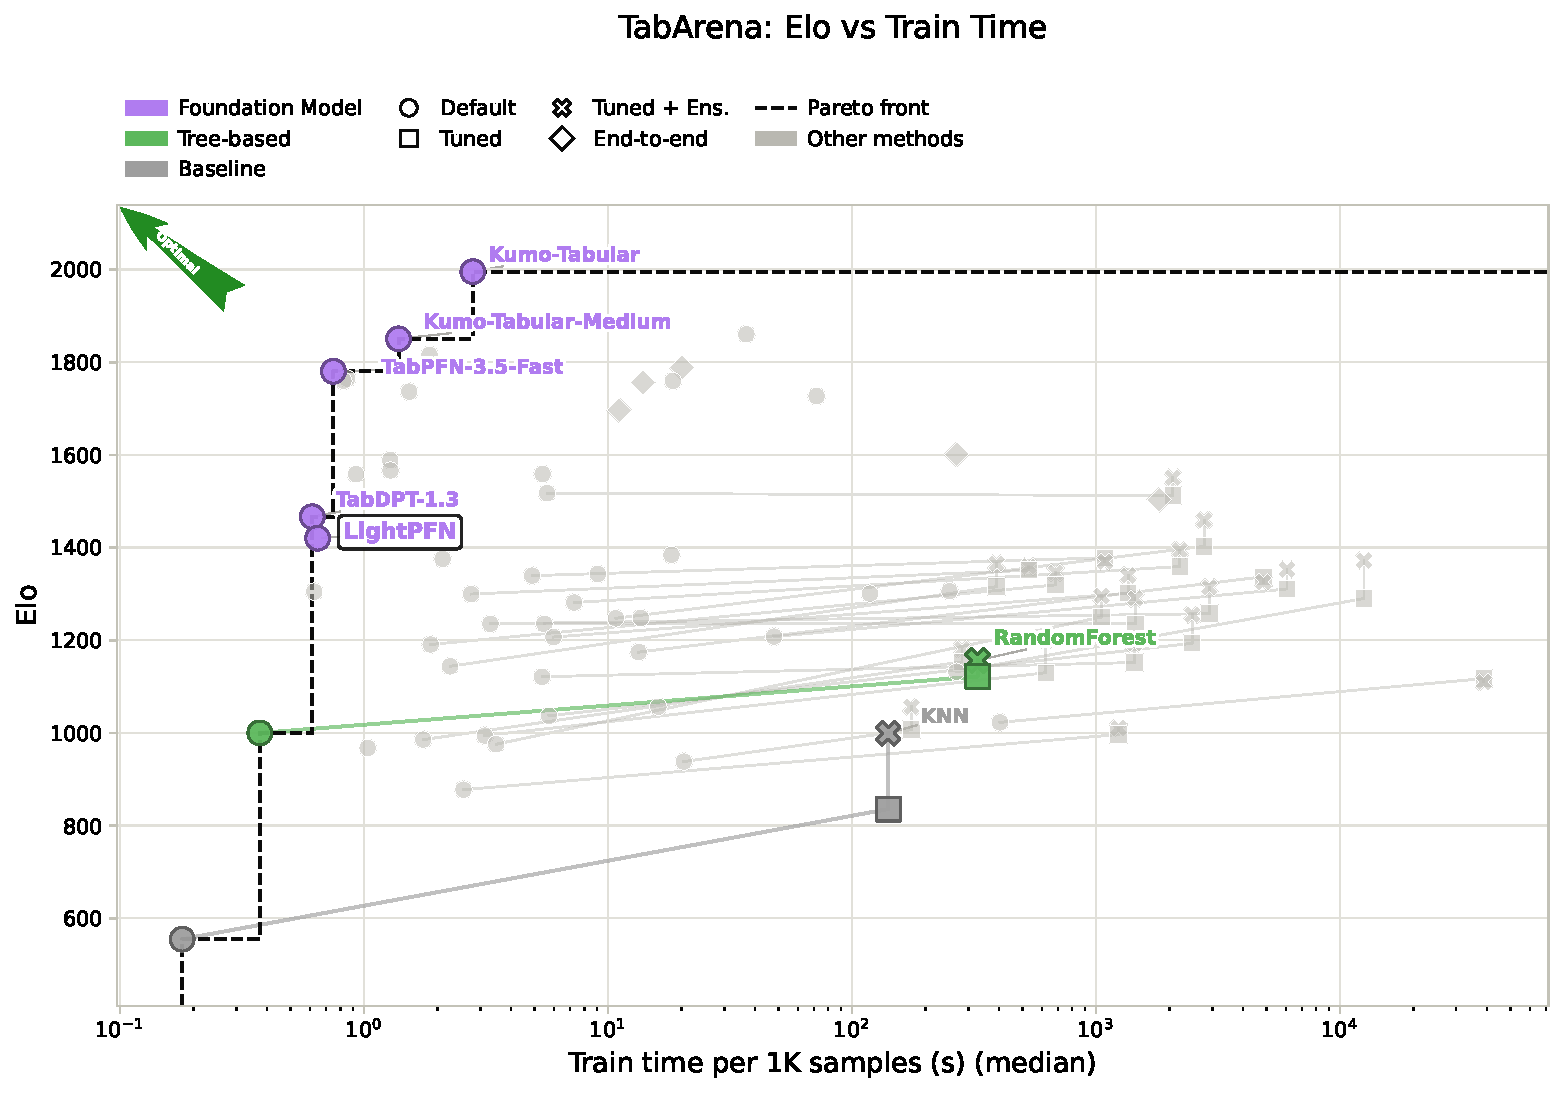
\includegraphics[width=\linewidth]{figures/official_lite_pareto.pdf}
\caption{Official TabArena-Lite classification: Elo against median fit time per 1,000 rows, from the
leaderboard snapshot. LightPFN is highlighted in the foundation-model color. Hardware differs across methods.}
\label{fig:official-lite}
\end{figure}

\FloatBarrier
\section{Categorical features}
\label{sec:categorical}

LightPFN reads categorical columns as ordinal codes. Its largest TabArena losses are on mostly categorical tables
(Section~\ref{sec:tabarena}), and on D4 it trails default CatBoost on the datasets with categorical columns of
hundreds to thousands of levels (Section~\ref{sec:large}). Removing the categorical columns with more than 50
levels at 10,000 training rows measures what each model draws from them (Table~\ref{tab:hicard}): CatBoost loses
0.4 to 2.0 AUC points, 1.0 on average, and LightPFN 0.2 on average. On one synthetic lookup column the model keeps
pace with CatBoost up to 500 categories (AUC 0.881 against 0.885) and falls behind at 2,000 (0.864 against 0.892).
Recognizing a category is therefore not the difficulty; using many rare categories, each with a small effect of
its own, is.

\begin{table}[t]
\centering
\footnotesize
\begin{tabular}{lccc}
\toprule
dataset & columns $>$50 levels (largest) & LightPFN gain & CatBoost gain \\
\midrule
airlines & 2 (266) & $+0.54$ & $+1.02$ \\
albert & 36 (6,006) & $+0.17$ & $+1.12$ \\
kick & 5 (711) & $+0.07$ & $+0.36$ \\
okcupid-stem & 3 (1,951) & $+0.29$ & $+0.92$ \\
sf-police-incidents & 1 (5,206) & $+0.49$ & $+2.02$ \\
porto-seguro & 1 (104) & $-0.28$ & $+0.42$ \\
\bottomrule
\end{tabular}
\caption{AUC points each model gains from the categorical columns with more than 50 levels: AUC with all
columns minus AUC without those columns, D4 datasets at 10,000 training rows, LightPFN with one estimator and
the whole training set as context, CatBoost at default settings.}
\label{tab:hicard}
\end{table}

We tested three remedies that keep the pretrained weights. Selection used D3 and Dcat, the twelve cells
formed by the six D4 datasets with categorical columns of more than two levels at 10,000 and 25,000 training rows;
Dcat extends the protocol of Section~\ref{sec:eval} outside TabArena.
\begin{enumerate}
\item Thirteen inference-time encodings on D3: frequency encoding, one-hot encoding up to 16 levels,
random category codes, smoothed target encoding and leave-one-out statistics, used alone or alongside the
ordinal codes. None yields a mean AUC gain with an interval above zero. Target encodings lose 0.3 to 0.5 points.
Leave-one-out statistics tie each context row's feature to its own label and cause a collapse of about
12 AUC points.
\item The count columns of Kumo Tabular \cite{kumo}, one $\log(1+\mathrm{count})$ column per categorical column
with more than 50 levels: $+0.03$ points $[-0.19,\ 0.23]$ on Dcat.
\item A categorical adapter of 6,384 parameters: separate Fourier frequencies and projection for categorical
cells, as in Kumo Tabular, and the ordered target statistics of CatBoost \cite{prokhorenkova2018} for every
categorical cell, embedded through the label embedding of the column stage, plus count features. A context row
uses only the context rows that precede it in a random order, so its own label never enters its statistics;
query rows use all context rows. The adapter starts as the identity, and tables without categorical columns get
the released predictions bit for bit. Fine-tuned with all other weights frozen, it does not improve Dcat:
$-0.06$ points $[-0.22,\ 0.07]$ after 4,000 steps on pretraining-size tables of graph v4 and rule tasks, and
after 1,000 steps on a mix in which 60\% of the tasks have 1,024 to 10,240 rows, $+0.01$ $[-0.06,\ 0.08]$ for the
moving average and $-0.20$ $[-0.38,\ -0.04]$ for the raw weights.
\end{enumerate}
The mechanism works: gradients reach the adapter, the statistics match a direct computation and leak no label.
The limit is the prior. A high-cardinality column of graph v4 is a quantized numeric variable with permuted codes,
which the frozen network already exploits, so per-category statistics do not lower the training loss; the real
columns where CatBoost gains have many rare levels with small effects of their own, and no prior task resembles
them. Version 2 will add native categorical handling at pretraining time: the categorical mask as a model input
from the start and a prior family of categorical random effects. The adapter stays in the code, off by default.

\FloatBarrier
\section{Discussion and limitations}

\paragraph{Interactions.} The rule prior and the complete B4 configuration are complementary on the
mechanism probes. This supports preserving feature interactions before compression, but neither
isolates the row and column refinement effects nor measures how frequent pure interactions are in
real datasets.

\paragraph{Long contexts.} Further training improves larger-table performance without increasing the
parameter count. Most gains arrive early, including before the longest tables enter training; the
experiment therefore does not isolate context length from additional optimization. Remaining losses
concentrate on a few datasets, and inference retains a quadratic context-attention term. Training beyond
60,000 rows and inference in the 300,000-row regime remain untested.

\paragraph{Categorical inputs.} Several of the largest TabArena losses occur on mostly categorical
tables, and on large tables CatBoost draws much more from high-cardinality columns. Section~\ref{sec:categorical}
shows that neither encodings nor an adapter on the frozen network recover that signal; the evidence points at the
prior, which has to be tested by pretraining with categorical random effects.

\paragraph{Cost.} A small parameter count does not remove the cost of attention over long contexts.
Cache blocking improves the cell stages, while context size and estimator count still govern substantial
work. The reported cross-host timings indicate a cost concern on larger tables; controlled measurements
on an idle laptop CPU are needed before claiming comparable latency to boosted trees. Reducing context
or estimator count would also change predictions and requires a separate accuracy evaluation.

\paragraph{Limitations.} All ablations use one training seed and 8,000 steps; the hardware anchor
illustrates a D3 shift of 0.3 points without a recipe change, rather than estimating run-to-run variance.
D3 follows a lite protocol
with at most 1,000 rows and 100 features. The scale test covers larger tables with only 15 datasets,
six of them at 16,000 and 32,000 rows, and it also guided the long-context stage; D4 has 13 datasets and one repeat,
and its intervals are wide. Baselines on D3 and
in the scale test use default hyperparameters and a single model, as do our TabArena harness runs. The
separate official Lite comparison includes tuned and ensembled entries, but only one split per classification
dataset and awaits the maintainers' full-benchmark verification. The final run is a single run, and its comparison with C2 mixes
longer training with the larger batch and fresh data. The TabArena evaluation covers the 38 classification
tasks only, with the first of three or ten repeats. On
D3 the XGBoost wrapper fails on one task, so its predictive comparison excludes that task from both models. Class counts above ten, exact feature-order
invariance, and the isolated effects of row and column refinement remain unverified.

\section{Conclusion}

LightPFN combines summary-mediated row refinement, a second column stage and a rule prior within a
4.60-million-parameter budget, using only synthetic training data. The final long-context model reaches
0.911 mean AUC on D3, 0.86 points above default CatBoost, and improves performance on larger tables
without a clear change on the small-table sets. On the scale test and D4, its mean differences from
default CatBoost have intervals that include zero at the larger training sizes; this does not establish
equivalence, and several datasets remain 1 to 4 AUC points behind.

On the 38 TabArena classification tasks and one repeat of the official splits, four estimators rank
second among seven evaluated configurations, behind TabICLv2, and have lower error than default
CatBoost on 76\% of tasks. This harness comparison uses fixed defaults. Separately, the official TabArena-Lite pipeline places
LightPFN 25th of 99 entries with Elo 1420 ($+67/-66$), above the GBDT point estimates, with overlapping
intervals against tuned CatBoost. The full maintainer verification remains pending.
Cache blocking and folded normalization improve CPU inference time by up to 4.1 times without changing
predictions beyond floating-point rounding, and a Vulkan backend runs the same network on GPUs of any vendor.
Competitive latency against boosted trees on an idle laptop CPU remains to be measured. Code, weights and the
training pipeline are released under Apache 2.0 with a scikit-learn package. Version 2 will add native categorical
features, pretrained with a prior of high-cardinality categorical columns, and regression, within the same
parameter budget.

\section*{Declaration of generative AI and AI-assisted technologies}
During the preparation of this work the author used generative AI tools as coding and writing assistants: to
write and review parts of the code, to run and analyse experiments, and to draft and edit the text of this
report. The author reviewed and edited the results and the text as needed and takes full responsibility for the
content of this report.

\clearpage
\appendix
\section{Hyperparameters}

\begin{table}[h]
\centering
\small
\begin{tabular}{lp{0.74\linewidth}}
\toprule
Cell embedding & dimension 64; offsets $\{0,1,3\}$; 16 learned frequencies per offset; 4 rank frequencies \\
Column encoding & ISAB, 2 layers, 4 heads, 64 inducing tokens \\
Row refinement & $R=3$, $K=4$ temporary tokens; 4 broadcasts, 3 gathers, 4 heads \\
Column refinement & independent second ISAB stage, same dimensions as column encoding \\
Row compression & 4 separate readout tokens, 3 blocks, 4 heads; rotary positions on cell keys \\
ICL & 7 blocks (8 in A0), dimension 256, 8 heads, 1 key/value head for queries, 16 thinking rows \\
Decoder & retrieval attention, 4 heads, 16 label slots \\
MLP ratio & 2 everywhere \\
\midrule
Optimizers & Muon for block matrices, AdamW ($0.9$, $0.98$) elsewhere; weight decay 0.01 \\
Learning rate & $10^{-3}$, linear warmup, cosine to $10^{-4}$ \\
Ablations & 8,000 steps $\times$ 32 tasks, warmup 800 \\
Final run & 120,000 steps $\times$ 64 tasks, warmup 2,000, two GPUs \\
Long-context stage & from the final checkpoint; learning rate $10^{-4}$, warmup 200, cosine to $10^{-5}$;
  8 groups per GPU from pools of 256--2,048, 1,024--10,240 and 4,096--60,000 rows (15/35/50\% of the
  groups); micro-batch cost $n(m+8)\le1.1\times10^6$ with $m$ the real features, rows subsampled
  above it; 39,250 steps \\
Other & clip 1.0; EMA 0.999; bfloat16 autocast; $8\times10^5$ cells per micro-batch (final run) \\
Missingness & 30\% of tasks; MCAR, MAR, MNAR; rate $\mathrm{LogU}(0.01,0.5)$ per column \\
\bottomrule
\end{tabular}
\caption{Model and training hyperparameters. Series A and B used $4\times10^5$ cells per micro-batch
and series C $10^6$; the budget changes memory use while preserving the task-weighted objective,
up to floating-point accumulation effects.}
\end{table}

\begin{thebibliography}{99}\small

\bibitem{benjamini1995} Y.~Benjamini and Y.~Hochberg. Controlling the false discovery rate: a
practical and powerful approach to multiple testing. \emph{Journal of the Royal Statistical Society,
Series B}, 57(1):289--300, 1995.

\bibitem{bischl2021} B.~Bischl, G.~Casalicchio, M.~Feurer, P.~Gijsbers, F.~Hutter, M.~Lang,
R.~G.~Mantovani, J.~N.~van~Rijn, and J.~Vanschoren. OpenML benchmarking suites. In \emph{NeurIPS
Datasets and Benchmarks Track}, 2021.

\bibitem{breiman2001} L.~Breiman. Random forests. \emph{Machine Learning}, 45(1):5--32, 2001.

\bibitem{chen2016} T.~Chen and C.~Guestrin. XGBoost: a scalable tree boosting system. In
\emph{KDD}, 2016.

\bibitem{causilo} M.~Cho, M.~Jeong, D.~Lee, J.~Lee, and J.~Yoo. Causilo technical report.
arXiv:2609.22866v1, 2026. \url{https://arxiv.org/abs/2609.22866v1}.

\bibitem{darcet2024} T.~Darcet, M.~Oquab, J.~Mairal, and P.~Bojanowski. Vision transformers need
registers. In \emph{ICLR}, 2024.

\bibitem{tabarena} N.~Erickson, L.~Purucker, A.~Tschalzev, D.~Holzm\"uller, P.~M.~Desai,
D.~Salinas, and F.~Hutter. TabArena: a living benchmark for machine learning on tabular data. 2025.

\bibitem{geurts2006} P.~Geurts, D.~Ernst, and L.~Wehenkel. Extremely randomized trees. \emph{Machine
Learning}, 63(1):3--42, 2006.

\bibitem{hollmann2023} N.~Hollmann, S.~M\"uller, K.~Eggensperger, and F.~Hutter. TabPFN: a
transformer that solves small tabular classification problems in a second. In \emph{ICLR}, 2023.

\bibitem{hollmann2025} N.~Hollmann, S.~M\"uller, L.~Purucker, A.~Krishnakumar, M.~K\"orfer,
S.~B.~Hoo, R.~T.~Schirrmeister, and F.~Hutter. Accurate predictions on small data with a tabular
foundation model. \emph{Nature}, 637:319--326, 2025.

\bibitem{jordan2024} K.~Jordan, Y.~Jin, V.~Boza, J.~You, F.~Cesista, L.~Newhouse, and J.~Bernstein.
Muon: an optimizer for hidden layers in neural networks. Technical blog post, 2024.

\bibitem{ke2017} G.~Ke, Q.~Meng, T.~Finley, T.~Wang, W.~Chen, W.~Ma, Q.~Ye, and T.-Y.~Liu. LightGBM:
a highly efficient gradient boosting decision tree. In \emph{NeurIPS}, 2017.

\bibitem{lee2019} J.~Lee, Y.~Lee, J.~Kim, A.~Kosiorek, S.~Choi, and Y.~W.~Teh. Set Transformer: a
framework for attention-based permutation-invariant neural networks. In \emph{ICML}, 2019.

\bibitem{liu2025muon} J.~Liu et~al. Muon is scalable for LLM training. arXiv preprint, 2025.

\bibitem{loshchilov2019} I.~Loshchilov and F.~Hutter. Decoupled weight decay regularization. In
\emph{ICLR}, 2019.

\bibitem{muller2022} S.~M\"uller, N.~Hollmann, S.~Pineda~Arango, J.~Grabocka, and F.~Hutter.
Transformers can do Bayesian inference. In \emph{ICLR}, 2022.

\bibitem{kumo} NVIDIA. Kumo Tabular, reference implementation in structured-data-models, 2026.
\url{https://github.com/NVIDIA/structured-data-models}.

\bibitem{prokhorenkova2018} L.~Prokhorenkova, G.~Gusev, A.~Vorobev, A.~V.~Dorogush, and A.~Gulin.
CatBoost: unbiased boosting with categorical features. In \emph{NeurIPS}, 2018.

\bibitem{tabpfn3} Prior Labs. TabPFN-3: model release and technical documentation, 2026.

\bibitem{qu2025} J.~Qu, D.~Holzm\"uller, G.~Varoquaux, and M.~Le~Morvan. TabICL: a tabular foundation
model for in-context learning on large data. In \emph{ICML}, 2025.

\bibitem{tabiclv2} TabICLv2: technical report and reference implementation (tabicl 2.2.0),
2026.

\bibitem{shazeer2019} N.~Shazeer. Fast transformer decoding: one write-head is all you need. arXiv
preprint, 2019.

\bibitem{su2024} J.~Su, M.~Ahmed, Y.~Lu, S.~Pan, W.~Bo, and Y.~Liu. RoFormer: enhanced transformer
with rotary position embedding. \emph{Neurocomputing}, 568:127063, 2024.

\bibitem{tancik2020} M.~Tancik, P.~P.~Srinivasan, B.~Mildenhall, S.~Fridovich-Keil, N.~Raghavan,
U.~Singhal, R.~Ramamoorthi, J.~T.~Barron, and R.~Ng. Fourier features let networks learn high
frequency functions in low dimensional domains. In \emph{NeurIPS}, 2020.

\bibitem{limix} X.~Zhang et~al. LimiX: unleashing structured-data modeling capability for generalist
intelligence. arXiv preprint, 2025.

\bibitem{mitra} X.~Zhang et~al. Mitra: mixed synthetic priors for enhancing tabular foundation
models. 2025.

\end{thebibliography}

\end{document}
